% Generated by Sphinx.
\def\sphinxdocclass{report}
\documentclass[a4paper,10pt,english]{sphinxmanual}
\usepackage[utf8]{inputenc}
\DeclareUnicodeCharacter{00A0}{\nobreakspace}
\usepackage{cmap}
\usepackage[T1]{fontenc}
\usepackage{babel}
\usepackage{times}
\usepackage[Bjarne]{fncychap}
\usepackage{longtable}
\usepackage{sphinx}
\usepackage{multirow}

\addto\captionsenglish{\renewcommand{\figurename}{Fig. }}
\addto\captionsenglish{\renewcommand{\tablename}{Table }}
\floatname{literal-block}{Listing }



\title{EQcorrscan Documentation}
\date{November 23, 2015}
\release{0.0.9}
\author{Calum John Chamberlain}
\newcommand{\sphinxlogo}{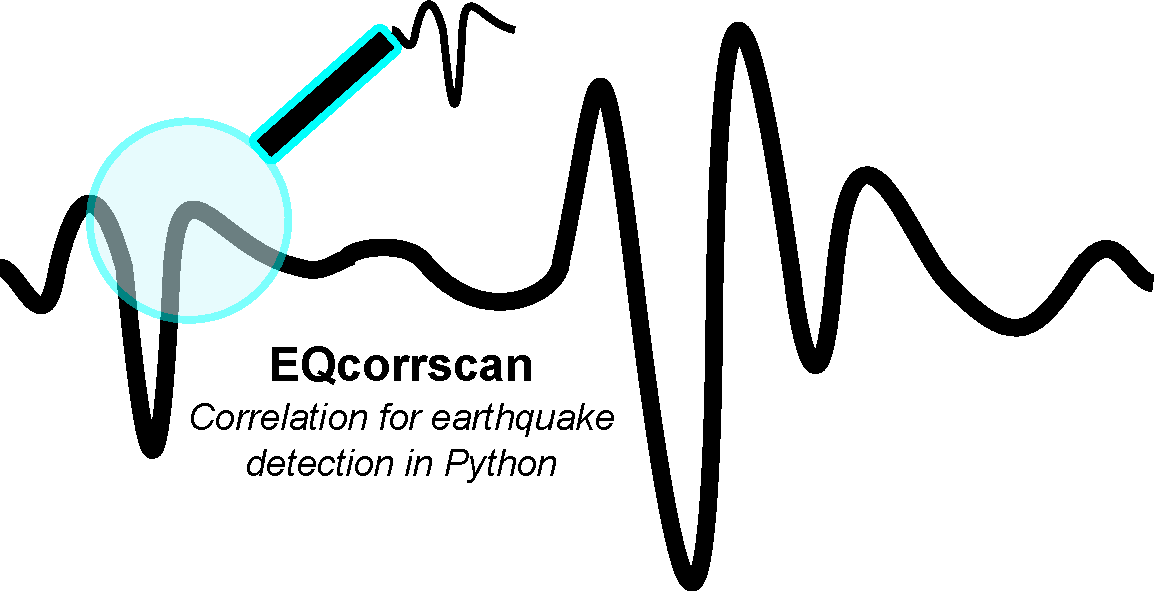
\includegraphics{EQcorrscan_logo.pdf}\par}
\renewcommand{\releasename}{Release}
\makeindex

\makeatletter
\def\PYG@reset{\let\PYG@it=\relax \let\PYG@bf=\relax%
    \let\PYG@ul=\relax \let\PYG@tc=\relax%
    \let\PYG@bc=\relax \let\PYG@ff=\relax}
\def\PYG@tok#1{\csname PYG@tok@#1\endcsname}
\def\PYG@toks#1+{\ifx\relax#1\empty\else%
    \PYG@tok{#1}\expandafter\PYG@toks\fi}
\def\PYG@do#1{\PYG@bc{\PYG@tc{\PYG@ul{%
    \PYG@it{\PYG@bf{\PYG@ff{#1}}}}}}}
\def\PYG#1#2{\PYG@reset\PYG@toks#1+\relax+\PYG@do{#2}}

\expandafter\def\csname PYG@tok@gd\endcsname{\def\PYG@tc##1{\textcolor[rgb]{0.63,0.00,0.00}{##1}}}
\expandafter\def\csname PYG@tok@gu\endcsname{\let\PYG@bf=\textbf\def\PYG@tc##1{\textcolor[rgb]{0.50,0.00,0.50}{##1}}}
\expandafter\def\csname PYG@tok@gt\endcsname{\def\PYG@tc##1{\textcolor[rgb]{0.00,0.27,0.87}{##1}}}
\expandafter\def\csname PYG@tok@gs\endcsname{\let\PYG@bf=\textbf}
\expandafter\def\csname PYG@tok@gr\endcsname{\def\PYG@tc##1{\textcolor[rgb]{1.00,0.00,0.00}{##1}}}
\expandafter\def\csname PYG@tok@cm\endcsname{\let\PYG@it=\textit\def\PYG@tc##1{\textcolor[rgb]{0.25,0.50,0.56}{##1}}}
\expandafter\def\csname PYG@tok@vg\endcsname{\def\PYG@tc##1{\textcolor[rgb]{0.73,0.38,0.84}{##1}}}
\expandafter\def\csname PYG@tok@m\endcsname{\def\PYG@tc##1{\textcolor[rgb]{0.13,0.50,0.31}{##1}}}
\expandafter\def\csname PYG@tok@mh\endcsname{\def\PYG@tc##1{\textcolor[rgb]{0.13,0.50,0.31}{##1}}}
\expandafter\def\csname PYG@tok@cs\endcsname{\def\PYG@tc##1{\textcolor[rgb]{0.25,0.50,0.56}{##1}}\def\PYG@bc##1{\setlength{\fboxsep}{0pt}\colorbox[rgb]{1.00,0.94,0.94}{\strut ##1}}}
\expandafter\def\csname PYG@tok@ge\endcsname{\let\PYG@it=\textit}
\expandafter\def\csname PYG@tok@vc\endcsname{\def\PYG@tc##1{\textcolor[rgb]{0.73,0.38,0.84}{##1}}}
\expandafter\def\csname PYG@tok@il\endcsname{\def\PYG@tc##1{\textcolor[rgb]{0.13,0.50,0.31}{##1}}}
\expandafter\def\csname PYG@tok@go\endcsname{\def\PYG@tc##1{\textcolor[rgb]{0.20,0.20,0.20}{##1}}}
\expandafter\def\csname PYG@tok@cp\endcsname{\def\PYG@tc##1{\textcolor[rgb]{0.00,0.44,0.13}{##1}}}
\expandafter\def\csname PYG@tok@gi\endcsname{\def\PYG@tc##1{\textcolor[rgb]{0.00,0.63,0.00}{##1}}}
\expandafter\def\csname PYG@tok@gh\endcsname{\let\PYG@bf=\textbf\def\PYG@tc##1{\textcolor[rgb]{0.00,0.00,0.50}{##1}}}
\expandafter\def\csname PYG@tok@ni\endcsname{\let\PYG@bf=\textbf\def\PYG@tc##1{\textcolor[rgb]{0.84,0.33,0.22}{##1}}}
\expandafter\def\csname PYG@tok@nl\endcsname{\let\PYG@bf=\textbf\def\PYG@tc##1{\textcolor[rgb]{0.00,0.13,0.44}{##1}}}
\expandafter\def\csname PYG@tok@nn\endcsname{\let\PYG@bf=\textbf\def\PYG@tc##1{\textcolor[rgb]{0.05,0.52,0.71}{##1}}}
\expandafter\def\csname PYG@tok@no\endcsname{\def\PYG@tc##1{\textcolor[rgb]{0.38,0.68,0.84}{##1}}}
\expandafter\def\csname PYG@tok@na\endcsname{\def\PYG@tc##1{\textcolor[rgb]{0.25,0.44,0.63}{##1}}}
\expandafter\def\csname PYG@tok@nb\endcsname{\def\PYG@tc##1{\textcolor[rgb]{0.00,0.44,0.13}{##1}}}
\expandafter\def\csname PYG@tok@nc\endcsname{\let\PYG@bf=\textbf\def\PYG@tc##1{\textcolor[rgb]{0.05,0.52,0.71}{##1}}}
\expandafter\def\csname PYG@tok@nd\endcsname{\let\PYG@bf=\textbf\def\PYG@tc##1{\textcolor[rgb]{0.33,0.33,0.33}{##1}}}
\expandafter\def\csname PYG@tok@ne\endcsname{\def\PYG@tc##1{\textcolor[rgb]{0.00,0.44,0.13}{##1}}}
\expandafter\def\csname PYG@tok@nf\endcsname{\def\PYG@tc##1{\textcolor[rgb]{0.02,0.16,0.49}{##1}}}
\expandafter\def\csname PYG@tok@si\endcsname{\let\PYG@it=\textit\def\PYG@tc##1{\textcolor[rgb]{0.44,0.63,0.82}{##1}}}
\expandafter\def\csname PYG@tok@s2\endcsname{\def\PYG@tc##1{\textcolor[rgb]{0.25,0.44,0.63}{##1}}}
\expandafter\def\csname PYG@tok@vi\endcsname{\def\PYG@tc##1{\textcolor[rgb]{0.73,0.38,0.84}{##1}}}
\expandafter\def\csname PYG@tok@nt\endcsname{\let\PYG@bf=\textbf\def\PYG@tc##1{\textcolor[rgb]{0.02,0.16,0.45}{##1}}}
\expandafter\def\csname PYG@tok@nv\endcsname{\def\PYG@tc##1{\textcolor[rgb]{0.73,0.38,0.84}{##1}}}
\expandafter\def\csname PYG@tok@s1\endcsname{\def\PYG@tc##1{\textcolor[rgb]{0.25,0.44,0.63}{##1}}}
\expandafter\def\csname PYG@tok@gp\endcsname{\let\PYG@bf=\textbf\def\PYG@tc##1{\textcolor[rgb]{0.78,0.36,0.04}{##1}}}
\expandafter\def\csname PYG@tok@sh\endcsname{\def\PYG@tc##1{\textcolor[rgb]{0.25,0.44,0.63}{##1}}}
\expandafter\def\csname PYG@tok@ow\endcsname{\let\PYG@bf=\textbf\def\PYG@tc##1{\textcolor[rgb]{0.00,0.44,0.13}{##1}}}
\expandafter\def\csname PYG@tok@sx\endcsname{\def\PYG@tc##1{\textcolor[rgb]{0.78,0.36,0.04}{##1}}}
\expandafter\def\csname PYG@tok@bp\endcsname{\def\PYG@tc##1{\textcolor[rgb]{0.00,0.44,0.13}{##1}}}
\expandafter\def\csname PYG@tok@c1\endcsname{\let\PYG@it=\textit\def\PYG@tc##1{\textcolor[rgb]{0.25,0.50,0.56}{##1}}}
\expandafter\def\csname PYG@tok@kc\endcsname{\let\PYG@bf=\textbf\def\PYG@tc##1{\textcolor[rgb]{0.00,0.44,0.13}{##1}}}
\expandafter\def\csname PYG@tok@c\endcsname{\let\PYG@it=\textit\def\PYG@tc##1{\textcolor[rgb]{0.25,0.50,0.56}{##1}}}
\expandafter\def\csname PYG@tok@mf\endcsname{\def\PYG@tc##1{\textcolor[rgb]{0.13,0.50,0.31}{##1}}}
\expandafter\def\csname PYG@tok@err\endcsname{\def\PYG@bc##1{\setlength{\fboxsep}{0pt}\fcolorbox[rgb]{1.00,0.00,0.00}{1,1,1}{\strut ##1}}}
\expandafter\def\csname PYG@tok@mb\endcsname{\def\PYG@tc##1{\textcolor[rgb]{0.13,0.50,0.31}{##1}}}
\expandafter\def\csname PYG@tok@ss\endcsname{\def\PYG@tc##1{\textcolor[rgb]{0.32,0.47,0.09}{##1}}}
\expandafter\def\csname PYG@tok@sr\endcsname{\def\PYG@tc##1{\textcolor[rgb]{0.14,0.33,0.53}{##1}}}
\expandafter\def\csname PYG@tok@mo\endcsname{\def\PYG@tc##1{\textcolor[rgb]{0.13,0.50,0.31}{##1}}}
\expandafter\def\csname PYG@tok@kd\endcsname{\let\PYG@bf=\textbf\def\PYG@tc##1{\textcolor[rgb]{0.00,0.44,0.13}{##1}}}
\expandafter\def\csname PYG@tok@mi\endcsname{\def\PYG@tc##1{\textcolor[rgb]{0.13,0.50,0.31}{##1}}}
\expandafter\def\csname PYG@tok@kn\endcsname{\let\PYG@bf=\textbf\def\PYG@tc##1{\textcolor[rgb]{0.00,0.44,0.13}{##1}}}
\expandafter\def\csname PYG@tok@o\endcsname{\def\PYG@tc##1{\textcolor[rgb]{0.40,0.40,0.40}{##1}}}
\expandafter\def\csname PYG@tok@kr\endcsname{\let\PYG@bf=\textbf\def\PYG@tc##1{\textcolor[rgb]{0.00,0.44,0.13}{##1}}}
\expandafter\def\csname PYG@tok@s\endcsname{\def\PYG@tc##1{\textcolor[rgb]{0.25,0.44,0.63}{##1}}}
\expandafter\def\csname PYG@tok@kp\endcsname{\def\PYG@tc##1{\textcolor[rgb]{0.00,0.44,0.13}{##1}}}
\expandafter\def\csname PYG@tok@w\endcsname{\def\PYG@tc##1{\textcolor[rgb]{0.73,0.73,0.73}{##1}}}
\expandafter\def\csname PYG@tok@kt\endcsname{\def\PYG@tc##1{\textcolor[rgb]{0.56,0.13,0.00}{##1}}}
\expandafter\def\csname PYG@tok@sc\endcsname{\def\PYG@tc##1{\textcolor[rgb]{0.25,0.44,0.63}{##1}}}
\expandafter\def\csname PYG@tok@sb\endcsname{\def\PYG@tc##1{\textcolor[rgb]{0.25,0.44,0.63}{##1}}}
\expandafter\def\csname PYG@tok@k\endcsname{\let\PYG@bf=\textbf\def\PYG@tc##1{\textcolor[rgb]{0.00,0.44,0.13}{##1}}}
\expandafter\def\csname PYG@tok@se\endcsname{\let\PYG@bf=\textbf\def\PYG@tc##1{\textcolor[rgb]{0.25,0.44,0.63}{##1}}}
\expandafter\def\csname PYG@tok@sd\endcsname{\let\PYG@it=\textit\def\PYG@tc##1{\textcolor[rgb]{0.25,0.44,0.63}{##1}}}

\def\PYGZbs{\char`\\}
\def\PYGZus{\char`\_}
\def\PYGZob{\char`\{}
\def\PYGZcb{\char`\}}
\def\PYGZca{\char`\^}
\def\PYGZam{\char`\&}
\def\PYGZlt{\char`\<}
\def\PYGZgt{\char`\>}
\def\PYGZsh{\char`\#}
\def\PYGZpc{\char`\%}
\def\PYGZdl{\char`\$}
\def\PYGZhy{\char`\-}
\def\PYGZsq{\char`\'}
\def\PYGZdq{\char`\"}
\def\PYGZti{\char`\~}
% for compatibility with earlier versions
\def\PYGZat{@}
\def\PYGZlb{[}
\def\PYGZrb{]}
\makeatother

\renewcommand\PYGZsq{\textquotesingle}

\begin{document}

\maketitle
\tableofcontents
\phantomsection\label{index::doc}

\href{https://github.com/calum-chamberlain/EQcorrscan/releases}{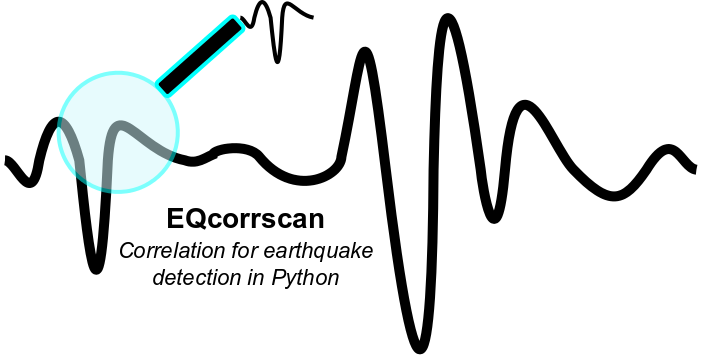
\includegraphics{EQcorrscan_logo.png}}

\chapter{EQcorrscan}
\label{index:eqcorrscan}\label{index:welcome-to-eqcorrscan-s-documentation}
A python package to conduct match-filter earthquake detections.  Codes are stored
on github, the bleeding edge master is \href{https://github.com/calum-chamberlain/EQcorrscan}{here}, or the latest stable(ish) release
can be found \href{https://github.com/calum-chamberlain/EQcorrscan/releases}{here}

This package contains routines to enable the user to conduct match-filter earthquake
detections using \href{https://github.com/obspy/obspy/wiki}{Obspy} bindings when reading
and writing seismic data, and the correlation routine in \href{http://opencv.org/}{openCV}.
Neither of these packages are installed by this software, due to a range of
licences being implimented.  However, both are open-source and should be installed
before using this package.  This package was written to impliment the matlab routines
used by Chamberlain et al. (2014) for the detection of low-frequency earthquakes.

Also within this package are:
\begin{itemize}
\item {} 
Clustering routines for seismic data;

\item {} 
Peak finding algorithm (basic);

\item {} 
Automatic amplitude picker for local magnitude scale;

\item {} 
\href{http://seisan.info/}{Seisan} S-file integration for database management and routine earthquake location;

\item {} 
Stacking routines including phase-weighted stacking based on Thurber at al. (2014);

\item {} 
Brightness based template creation based on the work of Frank et al. (2014)

\end{itemize}

This package is written by Calum Chamberlain of Victoria University of Wellington, and
is distributed under the LGPL GNU Licence, Copyright Calum Chamberlain 2015.


\chapter{References}
\label{index:references}\begin{itemize}
\item {} 
CJ Chamberlain, DR Shelly, J Townend, TA Stern (2014) \href{http://onlinelibrary.wiley.com/doi/10.1002/2014GC005436/full}{Low‐frequency earthquakes reveal punctuated slow slip on the deep extent of the Alpine Fault, New Zealand}, \emph{G-cubed}, doi:10.1002/2014GC005436

\item {} 
Thurber, C. H., Zeng, X., Thomas, A. M., \& Audet, P. (2014). \href{http://www.bssaonline.org/content/early/2014/08/12/0120140077.abstract}{Phase‐Weighted Stacking Applied to Low‐Frequency Earthquakes}, \emph{BSSA}, doi:10.1785/0120140077.

\item {} 
Frank, W. B., \& Shapiro, N. M. (2014). \href{http://gji.oxfordjournals.org/content/197/2/1215.short}{Automatic detection of low-frequency earthquakes (LFEs) based on a beamformed network response}, \emph{Geophysical Journal International}, 197(2), 1215-1223, doi:10.1093/gji/ggu058.

\end{itemize}


\chapter{Contents:}
\label{index:contents}

\section{Introduction to the EQcorrscan package}
\label{intro:introduction-to-the-eqcorrscan-package}\label{intro::doc}
This document is designed to give you an overview of the capabilities and
implementation of the EQcorrscan python module.


\subsection{Why EQcorrscan?}
\label{intro:why-eqcorrscan}
EQcorrscan is designed to compute matched-filter detections of earthquakes,
or any seismic signal (explosions work \emph{really} well) by comparing templates
with continuous data.  The main benefit of EQcorrscan is the level of
parallelisation that can be achieved.  By exploiting the fact that each template
does not rely on any other template, detections from a single template through
a day of seismic data can be computed in parallel.  By computing these in parallel
rather than a single template through multiple days we reduce IO load.  At a low
level, each time-step is computed in parallel by using the openCV matchTemplate
function.  The net result is that these functions are \emph{very} scalable, we have
obtained a speed-up from 2 months to 10 hours by migrating from a small cluster
to a large one (for a 6.5 year long continuous dataset and 800 templates).

The authors of EQcorrscan foresee this project as an open repository for the
development of software for the detection and analysis of repeating and
near-repeating earthquakes.  This repository will continue to grow and develop
and any and all help/criticism will be appreciated.

We have a long way to go with this project - if you want to get involved the
best place to start, and the most valuable thing for your understanding, and
for the health of this repository would be to contribute tests and
documentation.  Ideally we would like to have one test for every function!


\subsection{Installation}
\label{intro:installation}
A fresh install should be as simple as:

\textbf{pip install eqcorrscan}

Most codes should work without any effort on your part.  However you may need to
install the openCV-python package yourself.

This install has only been tested on Linux and OSX machines.  You
should be prepared for small differences in the results of your correlations
relating to foating-point truncation differences between 32 and 64-Bit
machines.

If you plan to run the bright\_lights or generating a synthetic grid of
templates you will need to have grid csv files, which the authors have
previously used NonLinLoc to generate.  This is not provided here and should
be sourced from \href{http://alomax.free.fr/nlloc/}{NonLinLoc} This will provide
the Grid2Time routine which is required to set-up a lag-time grid for your
velocity model.  You should read the NonLinLoc documentation for more
information regarding how this process works and the input files you are
required to give.


\subsection{Functions}
\label{intro:functions}
This package is divided into sub-directories of \emph{core} and \emph{utils}.  The
\emph{utils} directory contains simple functions for integration with
\href{http://seisan.info/}{seisan}, these are in the \emph{Sfile\_util.py}
module and functions therein which are essentially barebones and do not have the
full functionality that seisan can handle.  \emph{utils} also contains a simple
peak-finding algorithm \emph{find\_peaks.py} which looks for peaks within noisy data
above a certain threshold and within windows.  Many other functions have been
added to this module to handle the analysis of repeating and near-repeating
earthquakes, including stacking routines, clustering algorithms, magnitude
calculation both by amplitude picking and by singular value decomposition.  I
recommend you take a look in here to see if any of it is useful.  There are also
some plotting routines that make handling large datasets a little simpler.  Most
recently I have added a simple synthetic seismogram generator, which is currently
my main project focus.

Since earlier versions the \emph{core} modules have moved away from using parameter
files, and instead rely on explicit argument calls.  The parameter files are
still included by not documented here (see inside the par files), and remain
useful when generating batch scripts (see the scripts in the github repo).

Within \emph{core} you will find the core routines to generate templates,
\emph{(template\_gen)} search for likely templates \emph{(bright\_lights)} and
compute cross-channel correlations from these templates \emph{(match\_filter)}.  The
bright\_lights and match\_filter submodules have been designed with parallel
computing in mind, to the extent that the more cores and machines you have
running them the better.  These rely on the python multiprocesisng module to
handle parallelisation at lower-levels.  You can also do some `brute-force'
parallelisation on a day level when computing detections over multiple days.
I tend to run one day per node of a cluster computer, with each day running
templates in parallel.


\section{EQcorrscan tutorial}
\label{tutorial:eqcorrscan-tutorial}\label{tutorial::doc}
Welcome to EQcorrscan - this package is designed to compute earthquake detections
using a paralleled matched-filter network cross-correlation routine.  The inner
loop of this package is the cross-correlation of templates of seismic data
with day-ong seismic data.  This inner function is the openCV.match\_template
function - this appears to be a well optimized cross-correlation function, and
is written in c++.  Cross-correlations are computed in the frequency domain
for large datasets, for which a day of seismic data usually qualifies.

Before continuing with this tutorial please check that you have installed all
the pre-requisite modules, as not all will be installed by the setup.py file.
The list of these is in the Introduction section of this documentation.

As you will see, this package is divided into two main sub-modules, the
Core and Utils sub-modules.  The Core sub-module contains the main, high-level
functions:
\begin{quote}\begin{description}
\item[{bright\_lights}] \leavevmode
A brightness based template detection routine;

\item[{template\_gen}] \leavevmode
A series of routines to generate templates for match-filter detection
from continuous or cut data, with pick-times defined either manually, or from a
\emph{Seisan} s-file;

\item[{match\_filter}] \leavevmode
The main matched-filter routines, this is split into several
smaller functions to allow python based parallelisation;

\item[{lag\_calc}] \leavevmode
Routines for calculating optimal lag-times for events detected
by the match-filter routine, these lags can then be used to define new picks
for high accuracy relocations.

\end{description}\end{quote}

The Utils sub-module contains useful, but small functions.  These functions are
rarely cpu intensive, but perform vital operations, such as reading \emph{Seisan} s-files,
finding peaks in noisy data, converting a seisan database to hypoDD formatted
files and computing cross-correlations between detections for hypoDD (a double
difference reloaction software), calculating magnitudes, clustering detections,
stacking detections, making pretty plots, and processing seismic data in the
same way repeatedly using \emph{Obspy}`s functionality.


\subsection{Matched-filter detection}
\label{tutorial:matched-filter-detection}
In this section we will discuss generating a pair of templates from two
\emph{Seisan} s-files before using these templates to scan for similar earthquakes
within a day of data.  This small example does not truly exploit the parallel
operations within this package however, so you would be encouraged to think
about where parallel operations occur (\emph{hint, the code can run one template
per cpu}), and why there are --instance and--splits flags in the other
scripts in the guthub repository ({\color{red}\bfseries{}*}hint, if you have heaps of memory and cpus
\begin{quote}

you can do some brute force day parallelisation!*).
\end{quote}

The following script is included in the top-level directory alongside the full-scripts
used by the author to generate a 6.5 year long catalogue of low-frequency earthquakes
for the central Southern Alps of New Zealand.

This tutorial script highlights the ability of the match-filter method in detecting
earthquakes of near-repeating nature.  The dataset is a day of data taken from the
New Zealand national database, and the Southern Alp Microearthquake Borehole Array
(SAMBA) network (Boese et al. 2012).  This day was found to contain a swarm of
earthquakes, as published by Boese et al. (2014), the s-files provided are two
of these events.

The main processing flow is outlined in the figure below, note the main speedups
in this process are achieved by running multiple templates at once, however this
increases memory usage.  If memory is a problem there are flags (mem\_issue) in the
match\_filter.py source that can be turned on - the codes will then write temporary
files, which is slower, but can allow for more data crunching at once, your trade-off,
your call.

{\hfill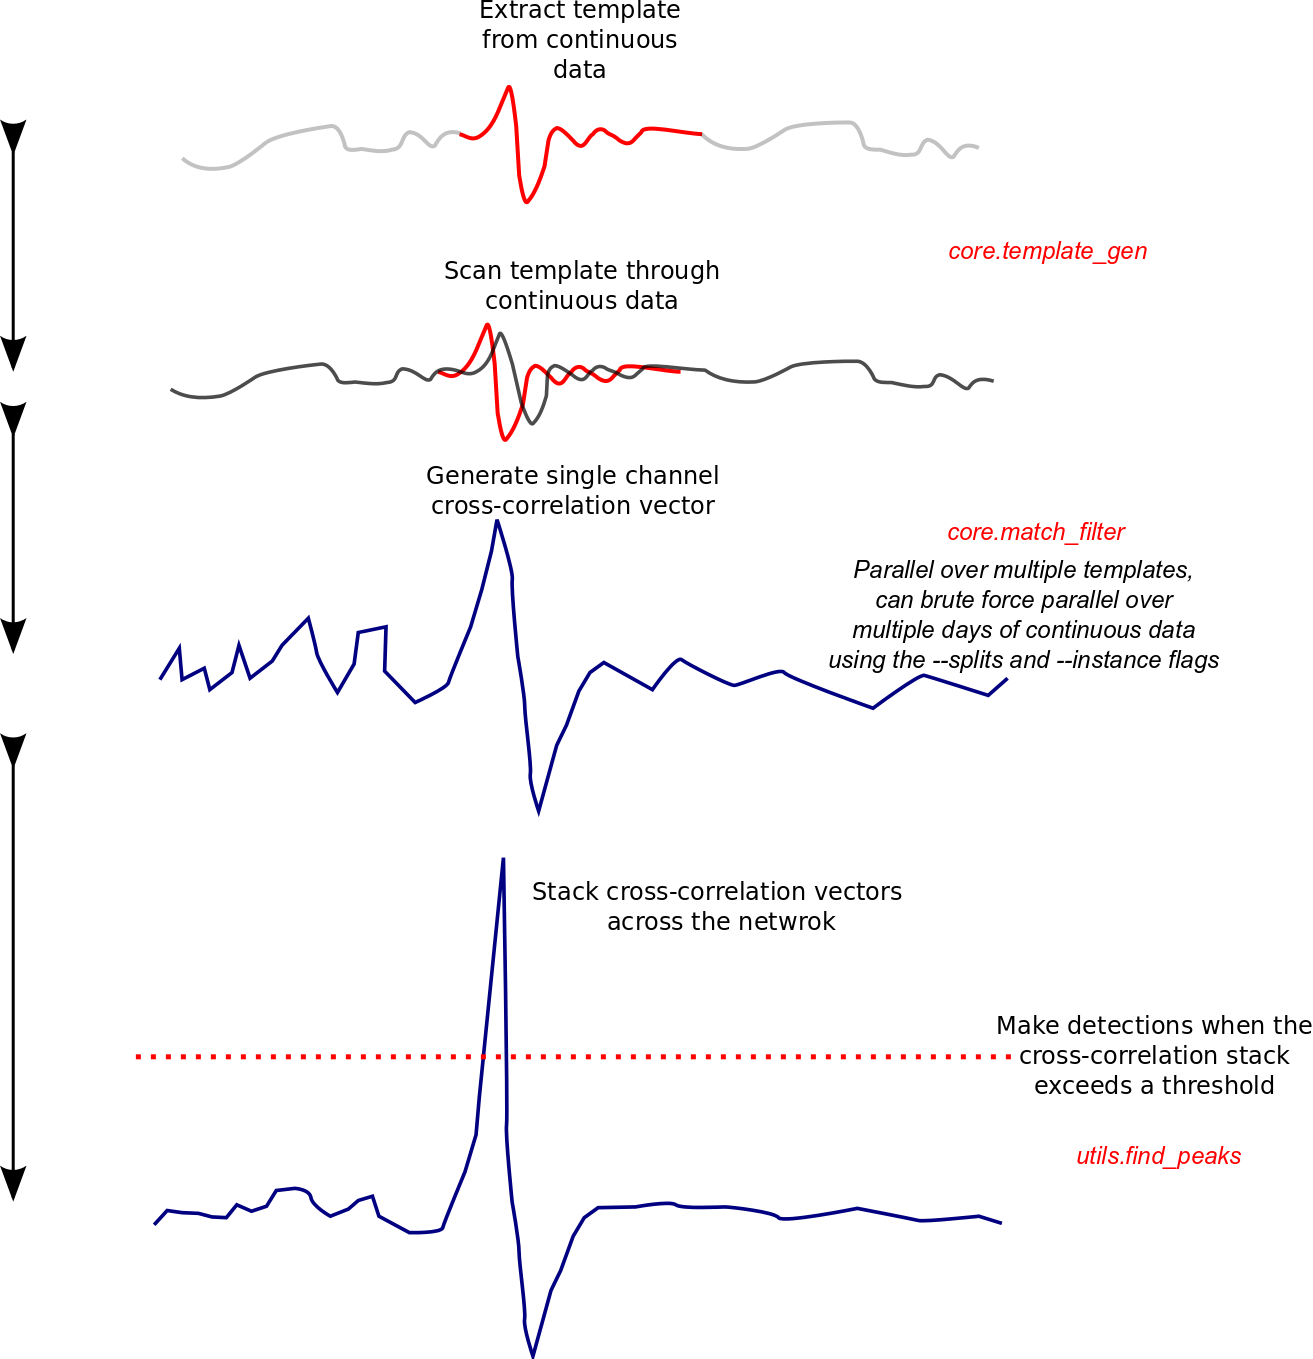
\includegraphics{processing_flow.png}\hfill}


\subsection{References}
\label{tutorial:references}\begin{itemize}
\item {} 
CM Boese, J Townend, E Smith, T Stern (2012). \href{http://onlinelibrary.wiley.com/doi/10.1029/2011JB008460/full}{Microseismicity and stress in the vicinity of the Alpine Fault, central Southern Alps, New Zealand}, \emph{JGR}, doi:10.1029/2011JB008460

\item {} 
CM Boese, KM Jacobs, EGC Smith, TA Stern, J Townend (2014). \href{http://onlinelibrary.wiley.com/doi/10.1002/2013GC005171/full}{Background and delayed-triggered swarms in the central Southern Alps, South Island, New Zealand}, \emph{G-cubed}, doi:10.1002/2013GC005171

\end{itemize}

\begin{Verbatim}[commandchars=\\\{\}]
\PYG{c}{\PYGZsh{}!/usr/bin/env python}
\PYG{l+s+sd}{r\PYGZdq{}\PYGZdq{}\PYGZdq{}Tutorial  This script is designed as a tutorial to highlight how to\PYGZbs{}}
\PYG{l+s+sd}{call the main functions within the EQcorrscan module.  In this tutorial}
\PYG{l+s+sd}{we will see how to generate a template and run this through the}
\PYG{l+s+sd}{matched\PYGZhy{}filter routine.}
\PYG{l+s+sd}{The template will be generated from a pre\PYGZhy{}picked earthquake, however there}
\PYG{l+s+sd}{are other ways to generate templates, for example this package also contains}
\PYG{l+s+sd}{a simple brightness function that is designed to scan continuous seismic}
\PYG{l+s+sd}{data and look for impulsive energy originating from a discrete point in a}
\PYG{l+s+sd}{seismic velocity model.}

\PYG{l+s+sd}{This package is dstributed under the LGPL v3.0, by using this script and the}
\PYG{l+s+sd}{functions contained within the EQcorrscan package you implicitly accept the}
\PYG{l+s+sd}{licence.  For the full wording of the licence refer to the licence.txt file.}

\PYG{l+s+sd}{Copyright 2015 Calum Chamberlain}

\PYG{l+s+sd}{This file is part of EQcorrscan.}

\PYG{l+s+sd}{    EQcorrscan is free software: you can redistribute it and/or modify}
\PYG{l+s+sd}{    it under the terms of the GNU General Public License as published by}
\PYG{l+s+sd}{    the Free Software Foundation, either version 3 of the License, or}
\PYG{l+s+sd}{    (at your option) any later version.}

\PYG{l+s+sd}{    EQcorrscan is distributed in the hope that it will be useful,}
\PYG{l+s+sd}{    but WITHOUT ANY WARRANTY; without even the implied warranty of}
\PYG{l+s+sd}{    MERCHANTABILITY or FITNESS FOR A PARTICULAR PURPOSE.  See the}
\PYG{l+s+sd}{    GNU General Public License for more details.}

\PYG{l+s+sd}{    You should have received a copy of the GNU General Public License}
\PYG{l+s+sd}{    along with EQcorrscan.  If not, see \PYGZlt{}http://www.gnu.org/licenses/\PYGZgt{}.}

\PYG{l+s+sd}{\PYGZdq{}\PYGZdq{}\PYGZdq{}}

\PYG{c}{\PYGZsh{} First we import the required modules:}
\PYG{k+kn}{import} \PYG{n+nn}{os}
\PYG{k+kn}{from} \PYG{n+nn}{obspy} \PYG{k+kn}{import} \PYG{n}{read}
\PYG{k+kn}{from} \PYG{n+nn}{obspy} \PYG{k+kn}{import} \PYG{n}{Stream}
\PYG{k+kn}{from} \PYG{n+nn}{eqcorrscan.core} \PYG{k+kn}{import} \PYG{n}{template\PYGZus{}gen}\PYG{p}{,} \PYG{n}{match\PYGZus{}filter}
\PYG{c}{\PYGZsh{} Before calling these module imports for parameter files you should insert}
\PYG{c}{\PYGZsh{} your own path into sys.path so that we find your parameter files.}
\PYG{k+kn}{from} \PYG{n+nn}{eqcorrscan.utils} \PYG{k+kn}{import} \PYG{n}{pre\PYGZus{}processing}\PYG{p}{,} \PYG{n}{Sfile\PYGZus{}util}
\PYG{k+kn}{import} \PYG{n+nn}{glob}

\PYG{c}{\PYGZsh{} Set up the default parameters \PYGZhy{} these used to be stored in parameter files}
\PYG{n}{debug} \PYG{o}{=} \PYG{l+m+mi}{3}  \PYG{c}{\PYGZsh{} High debug level should output lots to keep you informed}
\PYG{n}{threshold} \PYG{o}{=} \PYG{l+m+mf}{8.0}  \PYG{c}{\PYGZsh{} Threshold level as MAD multiplier}
\PYG{n}{threshtype} \PYG{o}{=} \PYG{l+s}{\PYGZsq{}}\PYG{l+s}{MAD}\PYG{l+s}{\PYGZsq{}}  \PYG{c}{\PYGZsh{} Threshold type, in this case Median Absolute Deviation}
\PYG{n}{trig\PYGZus{}int} \PYG{o}{=} \PYG{l+m+mf}{6.0}  \PYG{c}{\PYGZsh{} Minimum trigger interval for one template in seconds}

\PYG{c}{\PYGZsh{} Now we find the s\PYGZhy{}file we want to use to generate a template from}
\PYG{n}{data\PYGZus{}directory} \PYG{o}{=} \PYG{n}{os}\PYG{o}{.}\PYG{n}{path}\PYG{o}{.}\PYG{n}{join}\PYG{p}{(}\PYG{l+s}{\PYGZsq{}}\PYG{l+s}{test\PYGZus{}data}\PYG{l+s}{\PYGZsq{}}\PYG{p}{,} \PYG{l+s}{\PYGZsq{}}\PYG{l+s}{tutorial\PYGZus{}data}\PYG{l+s}{\PYGZsq{}}\PYG{p}{)}
\PYG{n}{sfiles} \PYG{o}{=} \PYG{n}{glob}\PYG{o}{.}\PYG{n}{glob}\PYG{p}{(}\PYG{n}{os}\PYG{o}{.}\PYG{n}{path}\PYG{o}{.}\PYG{n}{join}\PYG{p}{(}\PYG{n}{data\PYGZus{}directory}\PYG{p}{,} \PYG{l+s}{\PYGZsq{}}\PYG{l+s}{*L.S*}\PYG{l+s}{\PYGZsq{}}\PYG{p}{)}\PYG{p}{)}
\PYG{k}{print} \PYG{n}{sfiles}

\PYG{n}{templates} \PYG{o}{=} \PYG{p}{[}\PYG{p}{]}
\PYG{n}{template\PYGZus{}names} \PYG{o}{=} \PYG{p}{[}\PYG{p}{]}
\PYG{k}{for} \PYG{n}{i}\PYG{p}{,} \PYG{n}{sfile} \PYG{o+ow}{in} \PYG{n+nb}{enumerate}\PYG{p}{(}\PYG{n}{sfiles}\PYG{p}{)}\PYG{p}{:}
    \PYG{c}{\PYGZsh{} Read in the picks from the S\PYGZhy{}file, note, in the full case one fo the main\PYGZbs{}}
    \PYG{c}{\PYGZsh{} functions in template\PYGZus{}gen would be used rather than this, but for\PYGZbs{}}
    \PYG{c}{\PYGZsh{} the tutorial we will read in the data here \PYGZhy{} also note that this\PYGZbs{}}
    \PYG{c}{\PYGZsh{} template generation is inefficient for multiple templates, if using\PYGZbs{}}
    \PYG{c}{\PYGZsh{} daylong data for multiple templates you would want to only read\PYGZbs{}}
    \PYG{c}{\PYGZsh{} the seismic data once and cut it multiple times.}
    \PYG{n}{picks}\PYG{o}{=}\PYG{n}{Sfile\PYGZus{}util}\PYG{o}{.}\PYG{n}{readpicks}\PYG{p}{(}\PYG{n}{sfile}\PYG{p}{)}
    \PYG{k}{for} \PYG{n}{pick} \PYG{o+ow}{in} \PYG{n}{picks}\PYG{p}{:}
        \PYG{k}{print} \PYG{n}{pick}
        \PYG{k}{if} \PYG{o+ow}{not} \PYG{l+s}{\PYGZsq{}}\PYG{l+s}{wavefiles}\PYG{l+s}{\PYGZsq{}} \PYG{o+ow}{in} \PYG{n+nb}{locals}\PYG{p}{(}\PYG{p}{)}\PYG{p}{:}
            \PYG{n}{wavefiles} \PYG{o}{=} \PYG{n}{glob}\PYG{o}{.}\PYG{n}{glob}\PYG{p}{(}\PYG{n}{os}\PYG{o}{.}\PYG{n}{path}\PYG{o}{.}\PYG{n}{join}\PYG{p}{(}\PYG{n}{data\PYGZus{}directory}\PYG{p}{,}
                                               \PYG{l+s}{\PYGZsq{}}\PYG{l+s}{.}\PYG{l+s}{\PYGZsq{}}\PYG{o}{.}\PYG{n}{join}\PYG{p}{(}\PYG{p}{[}\PYG{n}{pick}\PYG{o}{.}\PYG{n}{station}\PYG{p}{,} \PYG{l+s}{\PYGZsq{}}\PYG{l+s}{*}\PYG{l+s}{\PYGZsq{}}\PYG{p}{]}\PYG{p}{)}\PYG{p}{)}\PYG{p}{)}
        \PYG{k}{else}\PYG{p}{:}
            \PYG{n}{wavefiles} \PYG{o}{+}\PYG{o}{=} \PYG{n}{glob}\PYG{o}{.}\PYG{n}{glob}\PYG{p}{(}\PYG{n}{os}\PYG{o}{.}\PYG{n}{path}\PYG{o}{.}\PYG{n}{join}\PYG{p}{(}\PYG{n}{data\PYGZus{}directory}\PYG{p}{,}
                                                \PYG{l+s}{\PYGZsq{}}\PYG{l+s}{.}\PYG{l+s}{\PYGZsq{}}\PYG{o}{.}\PYG{n}{join}\PYG{p}{(}\PYG{p}{[}\PYG{n}{pick}\PYG{o}{.}\PYG{n}{station}\PYG{p}{,} \PYG{l+s}{\PYGZsq{}}\PYG{l+s}{*}\PYG{l+s}{\PYGZsq{}}\PYG{p}{]}\PYG{p}{)}\PYG{p}{)}\PYG{p}{)}
    \PYG{n}{wavefiles} \PYG{o}{=} \PYG{n+nb}{list}\PYG{p}{(}\PYG{n+nb}{set}\PYG{p}{(}\PYG{n}{wavefiles}\PYG{p}{)}\PYG{p}{)}
    \PYG{k}{for} \PYG{n}{wavefile} \PYG{o+ow}{in} \PYG{n}{wavefiles}\PYG{p}{:}
        \PYG{k}{print} \PYG{l+s}{\PYGZsq{}}\PYG{l+s}{ }\PYG{l+s}{\PYGZsq{}}\PYG{o}{.}\PYG{n}{join}\PYG{p}{(}\PYG{p}{[}\PYG{l+s}{\PYGZsq{}}\PYG{l+s}{Reading data from}\PYG{l+s}{\PYGZsq{}}\PYG{p}{,} \PYG{n}{wavefile}\PYG{p}{]}\PYG{p}{)}
        \PYG{k}{if} \PYG{l+s}{\PYGZsq{}}\PYG{l+s}{st}\PYG{l+s}{\PYGZsq{}} \PYG{o+ow}{not} \PYG{o+ow}{in} \PYG{n+nb}{locals}\PYG{p}{(}\PYG{p}{)}\PYG{p}{:}
            \PYG{n}{st} \PYG{o}{=} \PYG{n}{read}\PYG{p}{(}\PYG{n}{wavefile}\PYG{p}{)}
        \PYG{k}{else}\PYG{p}{:}
            \PYG{n}{st} \PYG{o}{+}\PYG{o}{=} \PYG{n}{read}\PYG{p}{(}\PYG{n}{wavefile}\PYG{p}{)}

    \PYG{n}{st} \PYG{o}{=} \PYG{n}{st}\PYG{o}{.}\PYG{n}{merge}\PYG{p}{(}\PYG{n}{fill\PYGZus{}value}\PYG{o}{=}\PYG{l+s}{\PYGZsq{}}\PYG{l+s}{interpolate}\PYG{l+s}{\PYGZsq{}}\PYG{p}{)}
    \PYG{n}{day} \PYG{o}{=} \PYG{n}{st}\PYG{p}{[}\PYG{l+m+mi}{0}\PYG{p}{]}\PYG{o}{.}\PYG{n}{stats}\PYG{o}{.}\PYG{n}{starttime}\PYG{o}{.}\PYG{n}{date}

    \PYG{c}{\PYGZsh{} Process the data with our required parameters}
    \PYG{k}{for} \PYG{n}{tr} \PYG{o+ow}{in} \PYG{n}{st}\PYG{p}{:}
        \PYG{n}{tr} \PYG{o}{=} \PYG{n}{pre\PYGZus{}processing}\PYG{o}{.}\PYG{n}{dayproc}\PYG{p}{(}\PYG{n}{tr}\PYG{p}{,} \PYG{l+m+mf}{1.0}\PYG{p}{,} \PYG{l+m+mf}{20.0}\PYG{p}{,} \PYG{l+m+mi}{3}\PYG{p}{,} \PYG{l+m+mf}{100.0}\PYG{p}{,}\PYGZbs{}
                                    \PYG{n}{debug}\PYG{p}{,} \PYG{n}{day}\PYG{p}{)}

    \PYG{c}{\PYGZsh{} Use the template generation function to cut our templates}
    \PYG{n}{template} \PYG{o}{=} \PYG{n}{template\PYGZus{}gen}\PYG{o}{.}\PYG{n}{\PYGZus{}template\PYGZus{}gen}\PYG{p}{(}\PYG{n}{picks}\PYG{p}{,} \PYG{n}{st}\PYG{p}{,} \PYG{n}{length}\PYG{o}{=}\PYG{l+m+mf}{1.0}\PYG{p}{,} \PYG{n}{swin}\PYG{o}{=}\PYG{l+s}{\PYGZsq{}}\PYG{l+s}{all}\PYG{l+s}{\PYGZsq{}}\PYG{p}{,}
                                          \PYG{n}{prepick}\PYG{o}{=}\PYG{l+m+mf}{0.1}\PYG{p}{,} \PYG{n}{plot}\PYG{o}{=}\PYG{n+nb+bp}{True}\PYG{p}{)}
    \PYG{c}{\PYGZsh{} This will generate an obspy.Stream object}
    \PYG{c}{\PYGZsh{} Append this Stream to the list of templates}
    \PYG{n}{templates} \PYG{o}{+}\PYG{o}{=} \PYG{p}{[}\PYG{n}{template}\PYG{p}{]}
    \PYG{n}{template\PYGZus{}names}\PYG{o}{.}\PYG{n}{append}\PYG{p}{(}\PYG{l+s}{\PYGZsq{}}\PYG{l+s}{\PYGZus{}}\PYG{l+s}{\PYGZsq{}}\PYG{o}{.}\PYG{n}{join}\PYG{p}{(}\PYG{p}{[}\PYG{l+s}{\PYGZsq{}}\PYG{l+s}{tutorial}\PYG{l+s}{\PYGZsq{}}\PYG{p}{,} \PYG{n+nb}{str}\PYG{p}{(}\PYG{n}{i}\PYG{p}{)}\PYG{p}{]}\PYG{p}{)}\PYG{p}{)}

    \PYG{c}{\PYGZsh{} Save template for later}
    \PYG{n}{template}\PYG{o}{.}\PYG{n}{write}\PYG{p}{(}\PYG{n}{os}\PYG{o}{.}\PYG{n}{path}\PYG{o}{.}\PYG{n}{join}\PYG{p}{(}\PYG{n}{data\PYGZus{}directory}\PYG{p}{,} \PYG{l+s}{\PYGZsq{}}\PYG{l+s}{\PYGZus{}}\PYG{l+s}{\PYGZsq{}}\PYG{o}{.}\PYG{n}{join}\PYG{p}{(}\PYG{p}{[}\PYG{n}{template\PYGZus{}names}\PYG{p}{[}\PYG{n}{i}\PYG{p}{]}\PYG{p}{,}
                                                          \PYG{l+s}{\PYGZsq{}}\PYG{l+s}{template.ms}\PYG{l+s}{\PYGZsq{}}\PYG{p}{]}\PYG{p}{)}\PYG{p}{)}\PYG{p}{,}
                   \PYG{n}{format}\PYG{o}{=}\PYG{l+s}{\PYGZsq{}}\PYG{l+s}{MSEED}\PYG{l+s}{\PYGZsq{}}\PYG{p}{)}
    \PYG{c}{\PYGZsh{} Delete excess information from memory If you are re\PYGZhy{}using this script}
    \PYG{c}{\PYGZsh{} with the same templates you should be able to comment out this loop}
    \PYG{c}{\PYGZsh{} once you have generated your templates once.}
    \PYG{k}{del} \PYG{n}{template}\PYG{p}{,} \PYG{n}{st}

\PYG{c}{\PYGZsh{} Extract the stations from the templates}
\PYG{k}{for} \PYG{n}{template} \PYG{o+ow}{in} \PYG{n}{templates}\PYG{p}{:}
    \PYG{k}{if} \PYG{o+ow}{not} \PYG{l+s}{\PYGZsq{}}\PYG{l+s}{stachans}\PYG{l+s}{\PYGZsq{}} \PYG{o+ow}{in} \PYG{n+nb}{locals}\PYG{p}{(}\PYG{p}{)}\PYG{p}{:}
        \PYG{n}{stachans} \PYG{o}{=} \PYG{p}{[}\PYG{p}{(}\PYG{n}{tr}\PYG{o}{.}\PYG{n}{stats}\PYG{o}{.}\PYG{n}{station}\PYG{p}{,} \PYG{n}{tr}\PYG{o}{.}\PYG{n}{stats}\PYG{o}{.}\PYG{n}{channel}\PYG{p}{)} \PYG{k}{for} \PYG{n}{tr} \PYG{o+ow}{in} \PYG{n}{template}\PYG{p}{]}
    \PYG{k}{else}\PYG{p}{:}
        \PYG{n}{stachans} \PYG{o}{+}\PYG{o}{=} \PYG{p}{[}\PYG{p}{(}\PYG{n}{tr}\PYG{o}{.}\PYG{n}{stats}\PYG{o}{.}\PYG{n}{station}\PYG{p}{,} \PYG{n}{tr}\PYG{o}{.}\PYG{n}{stats}\PYG{o}{.}\PYG{n}{channel}\PYG{p}{)} \PYG{k}{for} \PYG{n}{tr} \PYG{o+ow}{in} \PYG{n}{template}\PYG{p}{]}

\PYG{c}{\PYGZsh{} Make this a unique list}
\PYG{n}{stachans} \PYG{o}{=} \PYG{n+nb}{list}\PYG{p}{(}\PYG{n+nb}{set}\PYG{p}{(}\PYG{n}{stachans}\PYG{p}{)}\PYG{p}{)}

\PYG{c}{\PYGZsh{} Read in the continuous data for these station, channel combinations}
\PYG{k}{for} \PYG{n}{stachan} \PYG{o+ow}{in} \PYG{n}{stachans}\PYG{p}{:}
    \PYG{n}{data\PYGZus{}file} \PYG{o}{=} \PYG{l+s}{\PYGZsq{}}\PYG{l+s}{\PYGZsq{}}\PYG{o}{.}\PYG{n}{join}\PYG{p}{(}\PYG{p}{[}\PYG{n}{stachan}\PYG{p}{[}\PYG{l+m+mi}{0}\PYG{p}{]}\PYG{p}{,} \PYG{l+s}{\PYGZsq{}}\PYG{l+s}{.*..*}\PYG{l+s}{\PYGZsq{}}\PYG{p}{,} \PYG{n}{stachan}\PYG{p}{[}\PYG{l+m+mi}{1}\PYG{p}{]}\PYG{p}{[}\PYG{o}{\PYGZhy{}}\PYG{l+m+mi}{1}\PYG{p}{]}\PYG{p}{,} \PYG{l+s}{\PYGZsq{}}\PYG{l+s}{.*}\PYG{l+s}{\PYGZsq{}}\PYG{p}{]}\PYG{p}{)}
    \PYG{n}{data\PYGZus{}file} \PYG{o}{=} \PYG{n}{os}\PYG{o}{.}\PYG{n}{path}\PYG{o}{.}\PYG{n}{join}\PYG{p}{(}\PYG{n}{data\PYGZus{}directory}\PYG{p}{,} \PYG{n}{data\PYGZus{}file}\PYG{p}{)}
    \PYG{k}{print} \PYG{l+s}{\PYGZsq{}}\PYG{l+s}{ }\PYG{l+s}{\PYGZsq{}}\PYG{o}{.}\PYG{n}{join}\PYG{p}{(}\PYG{p}{[}\PYG{l+s}{\PYGZsq{}}\PYG{l+s}{Reading data from:}\PYG{l+s}{\PYGZsq{}}\PYG{p}{,} \PYG{n}{data\PYGZus{}file}\PYG{p}{]}\PYG{p}{)}
    \PYG{c}{\PYGZsh{} Generate a new stream object and add to it}
    \PYG{k}{if} \PYG{l+s}{\PYGZsq{}}\PYG{l+s}{st}\PYG{l+s}{\PYGZsq{}} \PYG{o+ow}{not} \PYG{o+ow}{in} \PYG{n+nb}{locals}\PYG{p}{(}\PYG{p}{)}\PYG{p}{:}
        \PYG{n}{st} \PYG{o}{=} \PYG{n}{read}\PYG{p}{(}\PYG{n}{data\PYGZus{}file}\PYG{p}{)}
    \PYG{k}{else}\PYG{p}{:}
        \PYG{n}{st} \PYG{o}{+}\PYG{o}{=} \PYG{n}{read}\PYG{p}{(}\PYG{n}{data\PYGZus{}file}\PYG{p}{)}

\PYG{c}{\PYGZsh{} Merge the data to account for miniseed files being written in chunks}
\PYG{c}{\PYGZsh{} We need continuous day\PYGZhy{}long data, so data are padded if there are gaps}
\PYG{n}{st} \PYG{o}{=} \PYG{n}{st}\PYG{o}{.}\PYG{n}{merge}\PYG{p}{(}\PYG{n}{fill\PYGZus{}value}\PYG{o}{=}\PYG{l+s}{\PYGZsq{}}\PYG{l+s}{interpolate}\PYG{l+s}{\PYGZsq{}}\PYG{p}{)}

\PYG{c}{\PYGZsh{} Work out what day we are working on, required as we will pad the data to be daylong}
\PYG{n}{day} \PYG{o}{=} \PYG{n}{st}\PYG{p}{[}\PYG{l+m+mi}{0}\PYG{p}{]}\PYG{o}{.}\PYG{n}{stats}\PYG{o}{.}\PYG{n}{starttime}\PYG{o}{.}\PYG{n}{date}

\PYG{c}{\PYGZsh{} Process the data in the same way as the template}
\PYG{k}{for} \PYG{n}{tr} \PYG{o+ow}{in} \PYG{n}{st}\PYG{p}{:}
    \PYG{n}{tr} \PYG{o}{=} \PYG{n}{pre\PYGZus{}processing}\PYG{o}{.}\PYG{n}{dayproc}\PYG{p}{(}\PYG{n}{tr}\PYG{p}{,} \PYG{l+m+mf}{1.0}\PYG{p}{,} \PYG{l+m+mf}{20.0}\PYG{p}{,} \PYG{l+m+mi}{3}\PYG{p}{,} \PYG{l+m+mf}{100.0}\PYG{p}{,}\PYGZbs{}
                                \PYG{n}{debug}\PYG{p}{,} \PYG{n}{day}\PYG{p}{)}

\PYG{c}{\PYGZsh{} Compute detections}
\PYG{n}{detections} \PYG{o}{=} \PYG{n}{match\PYGZus{}filter}\PYG{o}{.}\PYG{n}{match\PYGZus{}filter}\PYG{p}{(}\PYG{n}{template\PYGZus{}names}\PYG{p}{,} \PYG{n}{templates}\PYG{p}{,} \PYG{n}{st}\PYG{p}{,}
                                       \PYG{n}{threshold}\PYG{p}{,} \PYG{n}{threshtype}\PYG{p}{,} \PYG{n}{trig\PYGZus{}int}\PYG{p}{,}
                                       \PYG{n}{plotvar}\PYG{o}{=}\PYG{n+nb+bp}{True}\PYG{p}{,} \PYG{n}{cores}\PYG{o}{=}\PYG{l+m+mi}{2}\PYG{p}{,} \PYG{n}{tempdir}\PYG{o}{=}\PYG{n+nb+bp}{False}\PYG{p}{,}
                                       \PYG{n}{debug}\PYG{o}{=}\PYG{n}{debug}\PYG{p}{,} \PYG{n}{plot\PYGZus{}format}\PYG{o}{=}\PYG{l+s}{\PYGZsq{}}\PYG{l+s}{pdf}\PYG{l+s}{\PYGZsq{}}\PYG{p}{)}

\PYG{c}{\PYGZsh{} We now have a list of detections! We can output these to a file to check later}
\PYG{n}{f} \PYG{o}{=} \PYG{n+nb}{open}\PYG{p}{(}\PYG{l+s}{\PYGZsq{}}\PYG{l+s}{tutorial\PYGZus{}detections.csv}\PYG{l+s}{\PYGZsq{}}\PYG{p}{,} \PYG{l+s}{\PYGZsq{}}\PYG{l+s}{w}\PYG{l+s}{\PYGZsq{}}\PYG{p}{)}
\PYG{k}{for} \PYG{n}{detection} \PYG{o+ow}{in} \PYG{n}{detections}\PYG{p}{:}
    \PYG{n}{line} \PYG{o}{=} \PYG{l+s}{\PYGZsq{}}\PYG{l+s}{, }\PYG{l+s}{\PYGZsq{}}\PYG{o}{.}\PYG{n}{join}\PYG{p}{(}\PYG{p}{[}\PYG{n}{detection}\PYG{o}{.}\PYG{n}{template\PYGZus{}name}\PYG{p}{,} \PYG{n+nb}{str}\PYG{p}{(}\PYG{n}{detection}\PYG{o}{.}\PYG{n}{detect\PYGZus{}time}\PYG{p}{)}\PYG{p}{,}
                      \PYG{n+nb}{str}\PYG{p}{(}\PYG{n}{detection}\PYG{o}{.}\PYG{n}{detect\PYGZus{}val}\PYG{p}{)}\PYG{p}{,} \PYG{n+nb}{str}\PYG{p}{(}\PYG{n}{detection}\PYG{o}{.}\PYG{n}{threshold}\PYG{p}{)}\PYG{p}{,}
                      \PYG{n+nb}{str}\PYG{p}{(}\PYG{n}{detection}\PYG{o}{.}\PYG{n}{no\PYGZus{}chans}\PYG{p}{)}\PYG{p}{]}\PYG{p}{)}
    \PYG{n}{f}\PYG{o}{.}\PYG{n}{write}\PYG{p}{(}\PYG{n}{line}\PYG{p}{)}
    \PYG{k}{print} \PYG{n}{line}
    \PYG{n}{f}\PYG{o}{.}\PYG{n}{write}\PYG{p}{(}\PYG{n}{os}\PYG{o}{.}\PYG{n}{linesep}\PYG{p}{)}
\PYG{n}{f}\PYG{o}{.}\PYG{n}{close}\PYG{p}{(}\PYG{p}{)}
\end{Verbatim}


\section{Core}
\label{core:core}\label{core::doc}
Core programs for the EQcorrscan project.


\subsection{bright\_lights}
\label{submodules/core.bright_lights:bright-lights}\label{submodules/core.bright_lights::doc}\label{submodules/core.bright_lights:module-bright_lights}\index{bright\_lights (module)}
Code to determine the brightness function of seismic data according to athree-dimensional travel-time grid.  This travel-time grid should be generatedusing the grid2time function of the NonLinLoc package by Anthony Lomax whichcan be found here: \href{http://alomax.free.fr/nlloc/}{http://alomax.free.fr/nlloc/} and is not distributed withinthis package as this is a very useful stand-alone library for seismic eventlocation.

This code is based on the method of Frank \& Shapiro 2014.

Code generated by Calum John Chamberlain of Victoria University of Wellington,2015.
\paragraph{Note}
\begin{description}
\item[{Pre-requisites:}] \leavevmode\begin{itemize}
\item {} 
gcc             - for the installation of the openCV correlation routine

\item {} 
python-cv2      - Python bindings for the openCV routines

\item {} 
python-joblib   - used for parallel processing

\item {} \begin{description}
\item[{python-obspy    - used for lots of common seismological processing}] \leavevmode\begin{itemize}
\item {} \begin{description}
\item[{requires:}] \leavevmode\begin{itemize}
\item {} 
numpy

\item {} 
scipy

\item {} 
matplotlib

\end{itemize}

\end{description}

\end{itemize}

\end{description}

\item {} 
NonLinLoc       - used outside of all codes for travel-time generation

\end{itemize}

\end{description}

Copyright 2015 Calum Chamberlain

This file is part of EQcorrscan.
\begin{quote}

EQcorrscan is free software: you can redistribute it and/or modify
it under the terms of the GNU General Public License as published by
the Free Software Foundation, either version 3 of the License, or
(at your option) any later version.

EQcorrscan is distributed in the hope that it will be useful,
but WITHOUT ANY WARRANTY; without even the implied warranty of
MERCHANTABILITY or FITNESS FOR A PARTICULAR PURPOSE.  See the
GNU General Public License for more details.

You should have received a copy of the GNU General Public License
along with EQcorrscan.  If not, see \textless{}\href{http://www.gnu.org/licenses/}{http://www.gnu.org/licenses/}\textgreater{}.
\end{quote}
\index{\_cum\_net\_resp() (in module bright\_lights)}

\begin{fulllineitems}
\phantomsection\label{submodules/core.bright_lights:bright_lights._cum_net_resp}\pysiglinewithargsret{\code{bright\_lights.}\bfcode{\_cum\_net\_resp}}{\emph{node\_lis}, \emph{instance=0}}{}
Function to compute the cumulative network response by reading thesaved energy .npy files.
\begin{quote}\begin{description}
\item[{Parameters}] \leavevmode\begin{itemize}
\item {} 
\textbf{\texttt{node\_lis}} (\emph{np.ndarray}) -- List of nodes (ints) to read from

\item {} 
\textbf{\texttt{instance}} (\emph{Int}) -- Instance flag for parallelisation, defaults to 0.

\end{itemize}

\item[{Returns}] \leavevmode
np.ndarray cum\_net\_resp, list of indeces used

\end{description}\end{quote}

\end{fulllineitems}

\index{\_find\_detections() (in module bright\_lights)}

\begin{fulllineitems}
\phantomsection\label{submodules/core.bright_lights:bright_lights._find_detections}\pysiglinewithargsret{\code{bright\_lights.}\bfcode{\_find\_detections}}{\emph{cum\_net\_resp}, \emph{nodes}, \emph{threshold}, \emph{thresh\_type}, \emph{samp\_rate}, \emph{realstations}, \emph{length}}{}
Function to find detections within the cumulative network responseaccording to Frank et al. (2014).
\begin{quote}\begin{description}
\item[{Parameters}] \leavevmode\begin{itemize}
\item {} 
\textbf{\texttt{cum\_net\_resp}} (\emph{np.ndarray}) -- Array of cumulative network response for nodes

\item {} 
\textbf{\texttt{nodes}} (\emph{list of tuples}) -- Nodes associated with the source of energy in the

\end{itemize}

\end{description}\end{quote}

cum\_net\_resp
:type threshold: float
:param threshold: Threshold value
:type thresh\_type: str
:param thresh\_type: Either MAD (Median Absolute Deviation) or abs(absolute) or RMS (Root Mean Squared)
:type samp\_rate: float
:param samp\_rate: Sampling rate in Hz
:type realstations: list of str
:param realstations: List of stations used to make the cumulative networkresponse, will be reported in the DETECTION
:type length: float
:param length: Maximum length of peak to look for in seconds
\begin{quote}\begin{description}
\item[{Returns}] \leavevmode
detections as :class: DETECTION

\end{description}\end{quote}

\end{fulllineitems}

\index{\_node\_loop() (in module bright\_lights)}

\begin{fulllineitems}
\phantomsection\label{submodules/core.bright_lights:bright_lights._node_loop}\pysiglinewithargsret{\code{bright\_lights.}\bfcode{\_node\_loop}}{\emph{stations}, \emph{lags}, \emph{stream}, \emph{clip\_level}, \emph{i=0}, \emph{mem\_issue=False}, \emph{instance=0}, \emph{plot=False}}{}
Internal function to allow for parallelisation of brightness.
\begin{quote}\begin{description}
\item[{Parameters}] \leavevmode\begin{itemize}
\item {} 
\textbf{\texttt{stations}} (\href{https://docs.python.org/library/functions.html\#list}{\emph{list}}) -- List of stations to use.

\item {} 
\textbf{\texttt{lags}} (\emph{np.ndarray}) -- List of lags where lags{[}i{[}:{]}{]} are the lags for stations{[}i{]}.

\item {} 
\textbf{\texttt{stream}} -- Data stream to find the brightness for.

\item {} 
\textbf{\texttt{clip\_level}} (\href{https://docs.python.org/library/functions.html\#float}{\emph{float}}) -- Upper limit for energy as a multiplier to the mean

\end{itemize}

\end{description}\end{quote}

energy.
:type i: int
:param i: Index of loop for parallelisation.
:type mem\_issue: bool
:param mem\_issue: If True will write to disk rather than storing data inRAM.
:type instance: int
:param instance: instance for bulk parallelisation, only used ifmem\_issue=true.
:type plot: bool
:param plot: Turn plotting on or off, defaults to False.
\begin{quote}\begin{description}
\item[{Returns}] \leavevmode
(i, energy (np.ndarray))

\end{description}\end{quote}

\end{fulllineitems}

\index{\_read\_tt() (in module bright\_lights)}

\begin{fulllineitems}
\phantomsection\label{submodules/core.bright_lights:bright_lights._read_tt}\pysiglinewithargsret{\code{bright\_lights.}\bfcode{\_read\_tt}}{\emph{path}, \emph{stations}, \emph{phase}, \emph{phaseout='S'}, \emph{ps\_ratio=1.68}, \emph{lags\_switch=True}}{}
Function to read in .csv files of slowness generated from Grid2Time(part of NonLinLoc by Anthony Lomax) and convert this to a useful formathere.

It should be noted that this can read either P or S travel-time grids, not
both at the moment.
\begin{quote}\begin{description}
\item[{Parameters}] \leavevmode\begin{itemize}
\item {} 
\textbf{\texttt{path}} (\href{https://docs.python.org/library/functions.html\#str}{\emph{str}}) -- The path to the .csv Grid2Time outputs

\item {} 
\textbf{\texttt{stations}} (\href{https://docs.python.org/library/functions.html\#list}{\emph{list}}) -- List of station names to read slowness files for.

\item {} 
\textbf{\texttt{phaseout}} (\href{https://docs.python.org/library/functions.html\#str}{\emph{str}}) -- What phase to return the lagtimes in

\item {} 
\textbf{\texttt{ps\_ratio}} (\href{https://docs.python.org/library/functions.html\#float}{\emph{float}}) -- p to s ratio for coversion

\item {} 
\textbf{\texttt{lags\_switch}} (\emph{Bool}) -- Return lags or raw travel-times, if set to true willreturn lags.

\end{itemize}

\item[{Returns}] \leavevmode
list stations, list of lists of tuples nodes, 

\item[{Class}] \leavevmode
`numpy.array' lags station{[}1{]} refers to nodes{[}1{]} and 

\end{description}\end{quote}

lags{[}1{]} nodes{[}1{]}{[}1{]} refers to station{[}1{]} and lags{[}1{]}{[}1{]}nodes{[}n{]}{[}n{]} is a tuple of latitude, longitude and depth

\end{fulllineitems}

\index{\_resample\_grid() (in module bright\_lights)}

\begin{fulllineitems}
\phantomsection\label{submodules/core.bright_lights:bright_lights._resample_grid}\pysiglinewithargsret{\code{bright\_lights.}\bfcode{\_resample\_grid}}{\emph{stations}, \emph{nodes}, \emph{lags}, \emph{mindepth}, \emph{maxdepth}, \emph{corners}, \emph{resolution}}{}
Function to resample the lagtime grid to a given volume.  For use if the
grid from Grid2Time is too large or you want to run a faster, downsampled
scan.
\begin{quote}\begin{description}
\item[{Parameters}] \leavevmode
\textbf{\texttt{stations}} (\href{https://docs.python.org/library/functions.html\#list}{\emph{list}}) -- List of station names from in the form where stations{[}i{]}

\end{description}\end{quote}

refers to nodes{[}i{]}{[}:{]} and lags{[}i{]}{[}:{]}
:type nodes: list, tuple
:param nodes: List of node points where nodes{[}i{]} referes to stations{[}i{]}and nodes{[}:{]}{[}:{]}{[}0{]} is latitude in degrees, nodes{[}:{]}{[}:{]}{[}1{]} is longitude indegrees, nodes{[}:{]}{[}:{]}{[}2{]} is depth in km.
:type lags: :class: `numpy.array'
:param lags: Array of arrays where lags{[}i{]}{[}:{]} refers to stations{[}i{]}.lags{[}i{]}{[}j{]} should be the delay to the nodes{[}i{]}{[}j{]} for stations{[}i{]} inseconds.
:type mindepth: float
:param mindepth: Upper limit of volume
:type maxdepth: float
:param maxdepth: Lower limit of volume
:type corners: matplotlib.Path
:param corners: matplotlib path of the corners for the 2D polygon to cutto in lat and long
\begin{quote}\begin{description}
\item[{Returns}] \leavevmode
list stations, list of lists of tuples nodes, :class: 

\end{description}\end{quote}

`numpy.array' lags station{[}1{]} refers to nodes{[}1{]} and lags{[}1{]}nodes{[}1{]}{[}1{]} refers to station{[}1{]} and lags{[}1{]}{[}1{]}nodes{[}n{]}{[}n{]} is a tuple of latitude, longitude and depth.

\end{fulllineitems}

\index{\_rm\_similarlags() (in module bright\_lights)}

\begin{fulllineitems}
\phantomsection\label{submodules/core.bright_lights:bright_lights._rm_similarlags}\pysiglinewithargsret{\code{bright\_lights.}\bfcode{\_rm\_similarlags}}{\emph{stations}, \emph{nodes}, \emph{lags}, \emph{threshold}}{}
Function to remove those nodes that have a very similar network moveout
to another lag.

Will, for each node, calculate the difference in lagtime at each station
at every node, then sum these for each node to get a cumulative difference
in network moveout.  This will result in an array of arrays with zeros on
the diagonal.
\begin{quote}\begin{description}
\item[{Parameters}] \leavevmode
\textbf{\texttt{stations}} (\href{https://docs.python.org/library/functions.html\#list}{\emph{list}}) -- List of station names from in the form where stations{[}i{]}

\end{description}\end{quote}

refers to nodes{[}i{]}{[}:{]} and lags{[}i{]}{[}:{]}
:type nodes: list, tuple
:param nodes: List of node points where nodes{[}i{]} referes to stations{[}i{]}and nodes{[}:{]}{[}:{]}{[}0{]} is latitude in degrees, nodes{[}:{]}{[}:{]}{[}1{]} is longitude indegrees, nodes{[}:{]}{[}:{]}{[}2{]} is depth in km.
:type lags: :class: `numpy.array'
:param lags: Array of arrays where lags{[}i{]}{[}:{]} refers to stations{[}i{]}.lags{[}i{]}{[}j{]} should be the delay to the nodes{[}i{]}{[}j{]} for stations{[}i{]} inseconds
:type threhsold: float
:param threshold: Threshold for removal in seconds
\begin{quote}\begin{description}
\item[{Returns}] \leavevmode
list stations, list of lists of tuples nodes, :class: 

\end{description}\end{quote}

`numpy.array' lags station{[}1{]} refers to nodes{[}1{]} and lags{[}1{]}nodes{[}1{]}{[}1{]} refers to station{[}1{]} and lags{[}1{]}{[}1{]}nodes{[}n{]}{[}n{]} is a tuple of latitude, longitude and depth.

\end{fulllineitems}

\index{\_rms() (in module bright\_lights)}

\begin{fulllineitems}
\phantomsection\label{submodules/core.bright_lights:bright_lights._rms}\pysiglinewithargsret{\code{bright\_lights.}\bfcode{\_rms}}{\emph{array}}{}
Calculate RMS of array

\end{fulllineitems}

\index{brightness() (in module bright\_lights)}

\begin{fulllineitems}
\phantomsection\label{submodules/core.bright_lights:bright_lights.brightness}\pysiglinewithargsret{\code{bright\_lights.}\bfcode{brightness}}{\emph{stations, nodes, lags, stream, threshold, thresh\_type, template\_length, template\_saveloc, coherence\_thresh, coherence\_stations={[}'all'{]}, coherence\_clip=False, gap=2.0, clip\_level=100, instance=0, pre\_pick=0.2, plotsave=True, cores=1}}{}
Function to calculate the brightness function in terms of energy fora day of data over the entire network for a given grid of nodes.

Note data in stream must be all of the same length and have the same
sampling rates.
\begin{quote}\begin{description}
\item[{Parameters}] \leavevmode
\textbf{\texttt{stations}} (\href{https://docs.python.org/library/functions.html\#list}{\emph{list}}) -- List of station names from in the form where stations{[}i{]}

\end{description}\end{quote}

refers to nodes{[}i{]}{[}:{]} and lags{[}i{]}{[}:{]}
:type nodes: list, tuple
:param nodes: List of node points where nodes{[}i{]} referes to stations{[}i{]}and nodes{[}:{]}{[}:{]}{[}0{]} is latitude in degrees, nodes{[}:{]}{[}:{]}{[}1{]} is longitude indegrees, nodes{[}:{]}{[}:{]}{[}2{]} is depth in km.
:type lags: :class: `numpy.array'
:param lags: Array of arrays where lags{[}i{]}{[}:{]} refers to stations{[}i{]}.lags{[}i{]}{[}j{]} should be the delay to the nodes{[}i{]}{[}j{]} for stations{[}i{]} inseconds.
:type stream: :class: \emph{obspy.Stream}
:param data: Data through which to look for detections.
:type threshold: float
:param threshold: Threshold value for detection of template within thebrightness function
:type thresh\_type: str
:param thresh\_type: Either MAD or abs where MAD is the Median AbsoluteDeviation and abs is an absoulte brightness.
:type template\_length: float
:param template\_length: Length of template to extract in seconds
:type template\_saveloc: str
:param template\_saveloc: Path of where to save the templates.
:type coherence\_thresh: tuple of floats
:param coherence\_thresh: Threshold for removing incoherant peaks in the
\begin{quote}

network response, those below this will not be used as templates.Must be in the form of (a,b) where the coherence is given by:a-kchan/b where kchan is the number of channels used to computethe coherence
\end{quote}
\begin{quote}\begin{description}
\item[{Parameters}] \leavevmode\begin{itemize}
\item {} 
\textbf{\texttt{coherence\_stations}} (\href{https://docs.python.org/library/functions.html\#list}{\emph{list}}) -- List of stations to use in the coherancethresholding - defaults to `all' which uses all the stations.

\item {} 
\textbf{\texttt{coherence\_clip}} (\emph{Start and end in seconds of data to window around,defaults to False, which uses all the data given.}) -- tuple

\item {} 
\textbf{\texttt{pre\_pick}} (\href{https://docs.python.org/library/functions.html\#float}{\emph{float}}) -- Seconds before the detection time to include in template

\item {} 
\textbf{\texttt{plotsave}} (\href{https://docs.python.org/library/functions.html\#bool}{\emph{bool}}) -- Save or show plots, if False will try and show the plotson screen - as this is designed for bulk use this is set toTrue to save any plots rather than show them if you createthem - changes the backend of matplotlib, so if is set toFalse you will see NO PLOTS!

\item {} 
\textbf{\texttt{core}} -- Number of cores to use, defaults to 1.

\item {} 
\textbf{\texttt{clip\_level}} (\href{https://docs.python.org/library/functions.html\#float}{\emph{float}}) -- Multiplier applied to the mean deviation of the energyas an upper limit, used to remove spikes (earthquakes, lightning, electircal spikes) from the energy stack.

\item {} 
\textbf{\texttt{gap}} (\href{https://docs.python.org/library/functions.html\#float}{\emph{float}}) -- Minimum inter-event time in seconds for detections

\end{itemize}

\item[{Returns}] \leavevmode
list of templates as :class: \emph{obspy.Stream} objects

\end{description}\end{quote}

\end{fulllineitems}

\index{coherence() (in module bright\_lights)}

\begin{fulllineitems}
\phantomsection\label{submodules/core.bright_lights:bright_lights.coherence}\pysiglinewithargsret{\code{bright\_lights.}\bfcode{coherence}}{\emph{stream\_in, stations={[}'all'{]}, clip=False}}{}
Function to determine the average network coherence of a giventemplate or detection.  You will want your stream to contain onlysignal as noise will reduce the coherence (assuming it is incoherantrandom noise).
\begin{quote}\begin{description}
\item[{Parameters}] \leavevmode\begin{itemize}
\item {} 
\textbf{\texttt{stream}} (\emph{obspy.Stream}) -- The stream of seismic data you want to calculate thecoherence for.

\item {} 
\textbf{\texttt{stations}} (\emph{List of String}) -- List of stations to use for coherence, default is all

\item {} 
\textbf{\texttt{clip}} (\emph{Tuple of Float}) -- Default is to use all the data given - tuple of start and end in seconds from start of trace

\end{itemize}

\item[{Returns}] \leavevmode
float - coherence, int number of channels used

\end{description}\end{quote}

\end{fulllineitems}



\subsection{template\_gen}
\label{submodules/core.template_gen:template-gen}\label{submodules/core.template_gen::doc}\label{submodules/core.template_gen:module-template_gen}\index{template\_gen (module)}
Function to generate template waveforms and information to go with themfor the application of cross-correlation of seismic data for the detection of
\begin{quote}

repeating events.
\end{quote}

Part of the EQcorrscan module to read nordic format s-filesEQcorrscan is a python module designed to run match filter routines forseismology, within it are routines for integration to seisan and obspy.With obspy integration (which is necessary) all main waveform formats can beread in and output.

This main section contains a script, LFE\_search.py which demonstrates theusage of the built in functions from template generation from picked waveformsthrough detection by match filter of continuous data to the generation of lagtimes to be used for relative locations.

The match-filter routine described here was used a previous Matlab code forthe Chamberlain et al. 2014 G-cubed publication.  The basis for the lag-timegeneration section is outlined in Hardebeck \& Shelly 2011, GRL.

Code generated by Calum John Chamberlain of Victoria University of Wellington,2015.
\paragraph{Note}
\begin{description}
\item[{Pre-requisites:}] \leavevmode\begin{itemize}
\item {} 
gcc             - for the installation of the openCV correlation routine

\item {} 
python-cv2      - Python bindings for the openCV routines

\item {} 
python-joblib   - used for parallel processing

\item {} \begin{description}
\item[{python-obspy    - used for lots of common seismological processing}] \leavevmode\begin{itemize}
\item {} \begin{description}
\item[{requires:}] \leavevmode\begin{itemize}
\item {} 
numpy

\item {} 
scipy

\item {} 
matplotlib

\end{itemize}

\end{description}

\end{itemize}

\end{description}

\item {} 
NonLinLoc       - used outside of all codes for travel-time generation

\end{itemize}

\end{description}

Copyright 2015 Calum Chamberlain

This file is part of EQcorrscan.
\begin{quote}

EQcorrscan is free software: you can redistribute it and/or modify
it under the terms of the GNU General Public License as published by
the Free Software Foundation, either version 3 of the License, or
(at your option) any later version.

EQcorrscan is distributed in the hope that it will be useful,
but WITHOUT ANY WARRANTY; without even the implied warranty of
MERCHANTABILITY or FITNESS FOR A PARTICULAR PURPOSE.  See the
GNU General Public License for more details.

You should have received a copy of the GNU General Public License
along with EQcorrscan.  If not, see \textless{}\href{http://www.gnu.org/licenses/}{http://www.gnu.org/licenses/}\textgreater{}.
\end{quote}
\index{\_template\_gen() (in module template\_gen)}

\begin{fulllineitems}
\phantomsection\label{submodules/core.template_gen:template_gen._template_gen}\pysiglinewithargsret{\code{template\_gen.}\bfcode{\_template\_gen}}{\emph{picks}, \emph{st}, \emph{length}, \emph{swin}, \emph{prepick=0.05}, \emph{plot=False}}{}
Function to generate a cut template in the obspyStream class from a given set of picks and data, also in an obspy streamclass.  Should be given pre-processed data (downsampled and filtered)
\begin{quote}\begin{description}
\item[{Parameters}] \leavevmode\begin{itemize}
\item {} 
\textbf{\texttt{picks}} -- Picks to extract data around

\item {} 
\textbf{\texttt{st}} -- Stream to etract templates from

\item {} 
\textbf{\texttt{length}} (\href{https://docs.python.org/library/functions.html\#float}{\emph{float}}) -- Length of template in seconds

\item {} 
\textbf{\texttt{swin}} (\href{https://docs.python.org/library/string.html\#module-string}{\emph{string}}) -- P, S or all

\item {} 
\textbf{\texttt{prepick}} (\href{https://docs.python.org/library/functions.html\#float}{\emph{float}}) -- Length in seconds to extract before the pick timedefault is 0.05 seconds

\item {} 
\textbf{\texttt{plot}} (\href{https://docs.python.org/library/functions.html\#bool}{\emph{bool}}) -- To plot the template or not, default is True

\end{itemize}

\end{description}\end{quote}

\end{fulllineitems}

\index{extract\_from\_stack() (in module template\_gen)}

\begin{fulllineitems}
\phantomsection\label{submodules/core.template_gen:template_gen.extract_from_stack}\pysiglinewithargsret{\code{template\_gen.}\bfcode{extract\_from\_stack}}{\emph{stack}, \emph{template}, \emph{length}, \emph{pre\_pick}, \emph{pre\_pad}, \emph{Z\_include=False}, \emph{pre\_processed=True}, \emph{samp\_rate=False}, \emph{lowcut=False}, \emph{highcut=False}, \emph{filt\_order=False}}{}
Function to extract a new template from a stack of previous detections.
Requires the stack, the template used to make the detections for the stack,
and we need to know if the stack has been pre-processed.
\begin{quote}\begin{description}
\item[{Parameters}] \leavevmode
\textbf{\texttt{stack}} (\emph{:class:obspy.Stream}) -- Waveform stack from detections.  Can be of any length and

\end{description}\end{quote}

can have delays already included, or not.
:type template: :class:obspy.Stream
:param template: Template used to make the detections in the stack. Willuse the delays of this for the new template.
:type length: float
:param length: Length of new template in seconds
:type pre\_pick: float
:param pre\_pick: Extract additional data before the detection, seconds
:type pre\_pad: float
:param pre\_pad: Pad used in seconds when extracting the data, e.g. thetime before the detection extracted.  If usingclustering.extract\_detections this half the length of the extractedwaveform.
:type Z\_include: bool
:param Z\_include: If True will include any Z-channels even if there isno template for this channel, as long as there is a template for thisstation at a different channel.  If this is False and Z channels areincluded in the template Z channels will be included in the new\_templateanyway.
:type pre\_processed: bool
:param pre\_processed: Have the data been pre-processed, if True (default)
\begin{quote}

then we will only cut the data here.
\end{quote}
\begin{quote}\begin{description}
\item[{Parameters}] \leavevmode\begin{itemize}
\item {} 
\textbf{\texttt{samp\_rate}} (\href{https://docs.python.org/library/functions.html\#float}{\emph{float}}) -- If pre\_processed=False then this is required, desiredsampling rate in Hz, defaults to False.

\item {} 
\textbf{\texttt{lowcut}} (\href{https://docs.python.org/library/functions.html\#float}{\emph{float}}) -- If pre\_processed=False then this is required, lowcut in Hz,defaults to False

\item {} 
\textbf{\texttt{highcut}} (\href{https://docs.python.org/library/functions.html\#float}{\emph{float}}) -- If pre\_processed=False then this is required, highcut in

\end{itemize}

\end{description}\end{quote}

Hz, defaults to False
:type filt\_order: int
:param filt\_order: If pre\_processed=False then this is required, filter
\begin{quote}

order, defaults to False
\end{quote}
\begin{quote}\begin{description}
\item[{Returns}] \leavevmode
:class:obspy.Stream Newly cut template

\end{description}\end{quote}

\end{fulllineitems}

\index{from\_contbase() (in module template\_gen)}

\begin{fulllineitems}
\phantomsection\label{submodules/core.template_gen:template_gen.from_contbase}\pysiglinewithargsret{\code{template\_gen.}\bfcode{from\_contbase}}{\emph{sfile}, \emph{contbase\_list}, \emph{lowcut}, \emph{highcut}, \emph{samp\_rate}, \emph{filt\_order}, \emph{length}, \emph{prepick}, \emph{swin}, \emph{debug=0}}{}
Function to read in picks from sfile then generate the template fromthe picks within this and the wavefiles from the continous database ofday-long files.  Included is a section to sanity check that the files aredaylong and that they start at the start of the day.  You should ensurethis is the case otherwise this may alter your data if your data aredaylong but the headers are incorrectly set.
\begin{quote}\begin{description}
\item[{Parameters}] \leavevmode\begin{itemize}
\item {} 
\textbf{\texttt{sfile}} (\href{https://docs.python.org/library/string.html\#module-string}{\emph{string}}) -- sfilename must be the path to a seisan nordic type s-file containing waveform and pick information, all other arguments can be numbers save for swin which must be either P, S or all (case-sensitive).

\item {} 
\textbf{\texttt{contbase\_list}} (\emph{List of tuple of string}) -- List of tuples of the form

\end{itemize}

\end{description}\end{quote}

{[}'path', `type', `network'{]}.  Where path is the path to the continuousdatabase, type is the directory structure, which can be eitherYyyyy/Rjjj.01, which is the standard IRIS Year, julian day structure, or,yyyymmdd which is a single directory for every day.
:type lowcut: float
:param lowcut: Low cut (Hz), if set to None will look in template
\begin{quote}

defaults file
\end{quote}
\begin{quote}\begin{description}
\item[{Parameters}] \leavevmode\begin{itemize}
\item {} 
\textbf{\texttt{lowcut}} -- High cut (Hz), if set to None will look in templatedefaults file

\item {} 
\textbf{\texttt{samp\_rate}} (\href{https://docs.python.org/library/functions.html\#float}{\emph{float}}) -- New sampling rate in Hz, if set to None will look intemplate defaults file

\item {} 
\textbf{\texttt{filt\_order}} (\href{https://docs.python.org/library/functions.html\#int}{\emph{int}}) -- Filter level, if set to None will look intemplate defaults file

\item {} 
\textbf{\texttt{length}} (\href{https://docs.python.org/library/functions.html\#float}{\emph{float}}) -- Extract length in seconds, if None will look in templatedefaults file.

\item {} 
\textbf{\texttt{prepick}} (\href{https://docs.python.org/library/functions.html\#float}{\emph{float}}) -- Pre-pick time in seconds

\item {} 
\textbf{\texttt{swin}} (\href{https://docs.python.org/library/functions.html\#str}{\emph{str}}) -- Either `all', `P' or `S', to select which phases to output.

\item {} 
\textbf{\texttt{debug}} (\href{https://docs.python.org/library/functions.html\#int}{\emph{int}}) -- Level of debugging output, higher=more

\end{itemize}

\end{description}\end{quote}

\end{fulllineitems}

\index{from\_sfile() (in module template\_gen)}

\begin{fulllineitems}
\phantomsection\label{submodules/core.template_gen:template_gen.from_sfile}\pysiglinewithargsret{\code{template\_gen.}\bfcode{from\_sfile}}{\emph{sfile}, \emph{lowcut}, \emph{highcut}, \emph{samp\_rate}, \emph{filt\_order}, \emph{length}, \emph{swin}, \emph{debug=0}}{}
Function to read in picks from sfile then generate the template from the
picks within this and the wavefile found in the pick file.
\begin{quote}\begin{description}
\item[{Parameters}] \leavevmode
\textbf{\texttt{sfile}} (\href{https://docs.python.org/library/string.html\#module-string}{\emph{string}}) -- sfilename must be the

\end{description}\end{quote}

path to a seisan nordic type s-file containing waveform and pickinformation.
:type lowcut: float
:param lowcut: Low cut (Hz), if set to None will look in template
\begin{quote}

defaults file
\end{quote}
\begin{quote}\begin{description}
\item[{Parameters}] \leavevmode\begin{itemize}
\item {} 
\textbf{\texttt{lowcut}} -- High cut (Hz), if set to None will look in templatedefaults file

\item {} 
\textbf{\texttt{samp\_rate}} (\href{https://docs.python.org/library/functions.html\#float}{\emph{float}}) -- New sampling rate in Hz, if set to None will look intemplate defaults file

\item {} 
\textbf{\texttt{filt\_order}} (\href{https://docs.python.org/library/functions.html\#int}{\emph{int}}) -- Filter level, if set to None will look intemplate defaults file

\item {} 
\textbf{\texttt{swin}} (\href{https://docs.python.org/library/functions.html\#str}{\emph{str}}) -- Either `all', `P' or `S', to select which phases to output.

\item {} 
\textbf{\texttt{length}} (\href{https://docs.python.org/library/functions.html\#float}{\emph{float}}) -- Extract length in seconds, if None will look in templatedefaults file.

\item {} 
\textbf{\texttt{debug}} (\href{https://docs.python.org/library/functions.html\#int}{\emph{int}}) -- Debug level, higher number=more output.

\end{itemize}

\end{description}\end{quote}

\end{fulllineitems}



\subsection{match\_filter}
\label{submodules/core.match_filter::doc}\label{submodules/core.match_filter:match-filter}\label{submodules/core.match_filter:module-match_filter}\index{match\_filter (module)}
Function to cross-correlate templates generated by template\_gen functionwith data and output the detecitons.  The main component of this script is thenormxcorr2 function from the openCV image processing package.  This is ahighly optimized and accurate normalized cross-correlation routine.  Thedetails of this code can be found here:* \href{http://www.cs.ubc.ca/research/deaton/remarks\_ncc.html}{http://www.cs.ubc.ca/research/deaton/remarks\_ncc.html}The cpp code was first tested using the Matlab mex wrapper, and has since beenported to a python callable dynamic library.

Part of the EQcorrscan module to integrate seisan nordic files into a fullcross-channel correlation for detection routine.EQcorrscan is a python module designed to run match filter routines forseismology, within it are routines for integration to seisan and obspy.With obspy integration (which is necessary) all main waveform formats can beread in and output.

This main section contains a script, LFE\_search.py which demonstrates theusage of the built in functions from template generation from picked waveformsthrough detection by match filter of continuous data to the generation of lagtimes to be used for relative locations.

The match-filter routine described here was used a previous Matlab code forthe Chamberlain et al. 2014 G-cubed publication.  The basis for the lag-timegeneration section is outlined in Hardebeck \& Shelly 2011, GRL.

Code generated by Calum John Chamberlain of Victoria University of Wellington,2015.
\paragraph{Note}
\begin{description}
\item[{Pre-requisites:}] \leavevmode\begin{itemize}
\item {} 
gcc             - for the installation of the openCV correlation routine

\item {} 
python-cv2      - Python bindings for the openCV routines

\item {} 
python-joblib   - used for parallel processing

\item {} \begin{description}
\item[{python-obspy    - used for lots of common seismological processing}] \leavevmode\begin{itemize}
\item {} \begin{description}
\item[{requires:}] \leavevmode\begin{itemize}
\item {} 
numpy

\item {} 
scipy

\item {} 
matplotlib

\end{itemize}

\end{description}

\end{itemize}

\end{description}

\item {} 
NonLinLoc       - used outside of all codes for travel-time generation

\end{itemize}

\end{description}

Copyright 2015 Calum Chamberlain

This file is part of EQcorrscan.
\begin{quote}

EQcorrscan is free software: you can redistribute it and/or modify
it under the terms of the GNU General Public License as published by
the Free Software Foundation, either version 3 of the License, or
(at your option) any later version.

EQcorrscan is distributed in the hope that it will be useful,
but WITHOUT ANY WARRANTY; without even the implied warranty of
MERCHANTABILITY or FITNESS FOR A PARTICULAR PURPOSE.  See the
GNU General Public License for more details.

You should have received a copy of the GNU General Public License
along with EQcorrscan.  If not, see \textless{}\href{http://www.gnu.org/licenses/}{http://www.gnu.org/licenses/}\textgreater{}.
\end{quote}
\index{DETECTION (class in match\_filter)}

\begin{fulllineitems}
\phantomsection\label{submodules/core.match_filter:match_filter.DETECTION}\pysiglinewithargsret{\strong{class }\code{match\_filter.}\bfcode{DETECTION}}{\emph{template\_name}, \emph{detect\_time}, \emph{no\_chans}, \emph{detect\_val}, \emph{threshold}, \emph{typeofdet}, \emph{chans=None}}{}
Information required for a full detection based on cross-channelcorrelation sums.
\begin{description}
\item[{Attributes:}] \leavevmode\begin{quote}\begin{description}
\item[{type template\_name}] \leavevmode
str

\item[{param template\_name}] \leavevmode
The name of the template for which this

\end{description}\end{quote}

detection was made.
:type detect\_time: :class: `obspy.UTCDateTime'
:param detect\_time: Time of detection as an obspy UTCDateTime object
:type no\_chans: int
:param no\_chans: The number of channels for which the cross-channelcorrelation sum was calculated over.
:type chans: list of str
:param chans: List of stations for the detection
:type cccsum\_val: float
:param cccsum\_val: The raw value of the cross-channel correlation sumfor this detection.
:type threshold: float
:param threshold: The value of the threshold used for this detection,will be the raw threshold value related to the cccsum.
:type typeofdet: str
:param typeofdet: Type of detection, STA, corr, bright

\end{description}

\end{fulllineitems}

\index{\_channel\_loop() (in module match\_filter)}

\begin{fulllineitems}
\phantomsection\label{submodules/core.match_filter:match_filter._channel_loop}\pysiglinewithargsret{\code{match\_filter.}\bfcode{\_channel\_loop}}{\emph{templates}, \emph{stream}, \emph{cores=1}, \emph{debug=0}}{}
Loop to generate cross channel correaltion sums for a series of templateshands off the actual correlations to a sister function which can be run inparallel.
\begin{quote}\begin{description}
\item[{Parameters}] \leavevmode
\textbf{\texttt{templates}} -- A list of templates, where each one should be an

\end{description}\end{quote}

obspy.Stream object containing multiple traces of seismic data and therelevant header information.
:param stream: A single obspy.Stream object containing daylong seismicdata to be correlated through using the templates.  This is in effect theimage.
:type core: int
:param core: Number of cores to loop over
:type debug: int
:param debug: Debug level.
\begin{quote}\begin{description}
\item[{Returns}] \leavevmode
New list of :class: `numpy.array' objects.  These will contain

\end{description}\end{quote}

the correlation sums for each template for this day of data.
:return: list of ints as number of channels used for each cross-correlation

\end{fulllineitems}

\index{\_template\_loop() (in module match\_filter)}

\begin{fulllineitems}
\phantomsection\label{submodules/core.match_filter:match_filter._template_loop}\pysiglinewithargsret{\code{match\_filter.}\bfcode{\_template\_loop}}{\emph{template}, \emph{chan}, \emph{station}, \emph{channel}, \emph{debug=0}, \emph{i=0}}{}
Sister loop to handle the correlation of a single template (of multiplechannels) with a single channel of data.
\begin{quote}\begin{description}
\item[{Parameters}] \leavevmode
\textbf{\texttt{i}} (\href{https://docs.python.org/library/functions.html\#int}{\emph{int}}) -- Optional argument, used to keep track of which process is being

\end{description}\end{quote}

run.
\begin{quote}\begin{description}
\item[{Returns}] \leavevmode
tuple of (i,ccc) with ccc as an ndarray

\end{description}\end{quote}
\paragraph{Note}
\begin{description}
\item[{..This function currently assumes only one template-channel per}] \leavevmode
data-channel, while this is normal for a standard matched-filter routine,if we wanted to impliment a subspace detector, this would be the functionto change, I think.  E.g. where I currently take only the first matchingchannel, we could loop through all the matching channels and then sum thecorrelation sums - however I don't really understand how you detect basedon that.  More reading of the Harris document required.

\end{description}

\end{fulllineitems}

\index{match\_filter() (in module match\_filter)}

\begin{fulllineitems}
\phantomsection\label{submodules/core.match_filter:match_filter.match_filter}\pysiglinewithargsret{\code{match\_filter.}\bfcode{match\_filter}}{\emph{template\_names}, \emph{template\_list}, \emph{st}, \emph{threshold}, \emph{threshold\_type}, \emph{trig\_int}, \emph{plotvar}, \emph{plotdir='.'}, \emph{cores=1}, \emph{tempdir=False}, \emph{debug=0}, \emph{plot\_format='jpg'}}{}
Over-arching code to run the correlations of given templates with aday of seismic data and output the detections based on a given threshold.
\begin{quote}\begin{description}
\item[{Parameters}] \leavevmode\begin{itemize}
\item {} 
\textbf{\texttt{template\_names}} (\href{https://docs.python.org/library/functions.html\#list}{\emph{list}}) -- List of template names in the same order astemplate\_list

\item {} 
\textbf{\texttt{template\_list}} (\emph{list :class: `obspy.Stream'}) -- A list of templates of which each template is aStream of obspy traces containing seismic data and header information.

\item {} 
\textbf{\texttt{st}} -- An obspy.Stream object containing all the data available andrequired for the correlations with templates given.  For efficiencythis should contain no excess traces which are not in one or more ofthe templates.  This will now remove excess traces internally, butwill copy the stream and work on the copy, leaving your input streamuntouched.

\item {} 
\textbf{\texttt{threshold}} (\href{https://docs.python.org/library/functions.html\#float}{\emph{float}}) -- A threshold value set based on the threshold\_type

\item {} 
\textbf{\texttt{threshold\_type}} (\href{https://docs.python.org/library/functions.html\#str}{\emph{str}}) -- The type of threshold to be used, can be MAD,absolute or av\_chan\_corr.    MAD threshold is calculated as thethreshold*(median(abs(cccsum))) where cccsum is the cross-correlationsum for a given template. absolute threhsold is a true absolutethreshold based on the cccsum value av\_chan\_corr is based on the meanvalues of single-channel cross-correlations assuming all data arepresent as required for the template, e.g. av\_chan\_corr\_thresh=threshold*(cccsum/len(template)) wheretemplate is a single template from the input and the length is thenumber of channels within this template.

\item {} 
\textbf{\texttt{trig\_int}} (\href{https://docs.python.org/library/functions.html\#float}{\emph{float}}) -- Minimum gap between detections in seconds.

\item {} 
\textbf{\texttt{plotvar}} (\href{https://docs.python.org/library/functions.html\#bool}{\emph{bool}}) -- Turn plotting on or off

\item {} 
\textbf{\texttt{plotdir}} (\href{https://docs.python.org/library/functions.html\#str}{\emph{str}}) -- Path to plotting folder, plots will be output here,defaults to run location.

\item {} 
\textbf{\texttt{tempdir}} (\emph{String or False}) -- Directory to put temporary files, or False

\item {} 
\textbf{\texttt{cores}} (\href{https://docs.python.org/library/functions.html\#int}{\emph{int}}) -- Number of cores to use

\item {} 
\textbf{\texttt{debug}} (\href{https://docs.python.org/library/functions.html\#int}{\emph{int}}) -- Debug output level, the bigger the number, the more theoutput.

\end{itemize}

\item[{Returns}] \leavevmode
\begin{quote}\begin{description}
\item[{class}] \leavevmode
`DETECTIONS' detections for each channel formatted as

\end{description}\end{quote}


\item[{Class}] \leavevmode
`obspy.UTCDateTime' objects.

\end{description}\end{quote}
\paragraph{Note
Plotting within the match-filter routine uses the Agg backend withinteractive plotting turned off.  This is because the function isdesigned to work in bulk.  If you wish to turn interactive plotting onyou must import matplotlib in your script first, when you them importmatch\_filter you will get the warning that this call to matplotlib hasno effect, which will mean that match\_filter has not changed theplotting behaviour.}

\end{fulllineitems}

\index{normxcorr2() (in module match\_filter)}

\begin{fulllineitems}
\phantomsection\label{submodules/core.match_filter:match_filter.normxcorr2}\pysiglinewithargsret{\code{match\_filter.}\bfcode{normxcorr2}}{\emph{template}, \emph{image}}{}
Base function to call the c++ correlation routine from the openCV imageprocessing suite.  Requires you to have installed the openCV pythonbindings, which can be downloaded on Linux machines using:\textbf{sudo apt-get install python-openCV}.

Here we use the cv2.TM\_CCOEFF\_NORMED method within openCV to give thenormalized cross-correaltion.  Documentation on this function can befound here:

\textbf{http://docs.opencv.org/modules/imgproc/doc/object\_detection.html?highlight=matchtemplate\#cv2.matchTemplate}
\begin{quote}\begin{description}
\item[{Parameters}] \leavevmode\begin{itemize}
\item {} 
\textbf{\texttt{template}} -- Template array

\item {} 
\textbf{\texttt{image}} -- image to scan

\end{itemize}

\end{description}\end{quote}

the template through.  The order of these matters, if you put the templateafter the image you will get a reversed correaltion matrix
\begin{quote}\begin{description}
\item[{Returns}] \leavevmode
New :class: `numpy.array' object of the correlation values for

\end{description}\end{quote}

the correlation of the image with the template.

\end{fulllineitems}



\subsection{lag\_calc}
\label{submodules/core.lag_calc:lag-calc}\label{submodules/core.lag_calc::doc}\label{submodules/core.lag_calc:module-lag_calc}\index{lag\_calc (module)}
Functions to generate lag-times for events detected by correlation.

Part of the EQcorrscan module to integrate seisan nordic files into a full
cross-channel correlation for detection routine.
EQcorrscan is a python module designed to run match filter routines for
seismology, within it are routines for integration to seisan and obspy.
With obspy integration (which is necessary) all main waveform formats can be
read in and output.

This main section contains a script, LFE\_search.py which demonstrates the usage
of the built in functions from template generation from picked waveforms
through detection by match filter of continuous data to the generation of lag
times to be used for relative locations.

The match-filter routine described here was used a previous Matlab code for the
Chamberlain et al. 2014 G-cubed publication.  The basis for the lag-time
generation section is outlined in Hardebeck \& Shelly 2011, GRL.

Code generated by Calum John Chamberlain of Victoria University of Wellington,
2015.
\paragraph{Note}
\begin{description}
\item[{Pre-requisites:}] \leavevmode\begin{itemize}
\item {} 
gcc             - for the installation of the openCV correlation routine

\item {} 
python-cv2      - Python bindings for the openCV routines

\item {} 
python-joblib   - used for parallel processing

\item {} \begin{description}
\item[{python-obspy    - used for lots of common seismological processing}] \leavevmode\begin{itemize}
\item {} \begin{description}
\item[{requires:}] \leavevmode\begin{itemize}
\item {} 
numpy

\item {} 
scipy

\item {} 
matplotlib

\end{itemize}

\end{description}

\end{itemize}

\end{description}

\item {} 
NonLinLoc       - used outside of all codes for travel-time generation

\end{itemize}

\end{description}

Copyright 2015 Calum Chamberlain

This file is part of EQcorrscan.
\begin{quote}

EQcorrscan is free software: you can redistribute it and/or modify
it under the terms of the GNU General Public License as published by
the Free Software Foundation, either version 3 of the License, or
(at your option) any later version.

EQcorrscan is distributed in the hope that it will be useful,
but WITHOUT ANY WARRANTY; without even the implied warranty of
MERCHANTABILITY or FITNESS FOR A PARTICULAR PURPOSE.  See the
GNU General Public License for more details.

You should have received a copy of the GNU General Public License
along with EQcorrscan.  If not, see \textless{}\href{http://www.gnu.org/licenses/}{http://www.gnu.org/licenses/}\textgreater{}.
\end{quote}
\index{\_channel\_loop() (in module lag\_calc)}

\begin{fulllineitems}
\phantomsection\label{submodules/core.lag_calc:lag_calc._channel_loop}\pysiglinewithargsret{\code{lag\_calc.}\bfcode{\_channel\_loop}}{\emph{detection}, \emph{template}, \emph{i=0}}{}
Utility function to take a stream of data for the detected event and parse
the correct data to lag\_gen
\begin{quote}\begin{description}
\item[{Parameters}] \leavevmode\begin{itemize}
\item {} 
\textbf{\texttt{detection}} (\emph{obspy.Stream}) -- Stream of data for the slave event detected using     template

\item {} 
\textbf{\texttt{template}} (\emph{obspy.Stream}) -- Stream of data as the template for the detection.

\item {} 
\textbf{\texttt{i}} (\emph{int, optional}) -- Used to track which process has occured when running in parallel

\end{itemize}

\item[{Returns}] \leavevmode
picks, a tuple of (lag in s, cross-correlation value, station,     chan)

\end{description}\end{quote}

\end{fulllineitems}

\index{day\_loop() (in module lag\_calc)}

\begin{fulllineitems}
\phantomsection\label{submodules/core.lag_calc:lag_calc.day_loop}\pysiglinewithargsret{\code{lag\_calc.}\bfcode{day\_loop}}{\emph{detection\_streams}, \emph{template}}{}
Function to loop through multiple detections for one template - ostensibly
designed to run for the same day of data for I/O simplicity, but as you
are passing stream objects it could run for all the detections ever, as long
as you have the RAM!
\begin{quote}\begin{description}
\item[{Parameters}] \leavevmode\begin{itemize}
\item {} 
\textbf{\texttt{detection\_streams}} (\emph{List of obspy.Stream}) -- List of all the detections for this template that you
want to compute the optimum pick for.

\item {} 
\textbf{\texttt{template}} (\emph{obspy.Stream}) -- The original template used to detect the detections passed

\end{itemize}

\item[{Returns}] \leavevmode
lags - List of List of tuple: lags{[}i{]} corresponds to detection{[}i{]},
lags{[}i{]}{[}j{]} corresponds to a channel of detection{[}i{]}, within
this tuple is the lag (in seconds), normalised correlation,
station and channel.

\end{description}\end{quote}

\end{fulllineitems}

\index{lag\_calc() (in module lag\_calc)}

\begin{fulllineitems}
\phantomsection\label{submodules/core.lag_calc:lag_calc.lag_calc}\pysiglinewithargsret{\code{lag\_calc.}\bfcode{lag\_calc}}{\emph{detections}, \emph{detect\_data}, \emph{templates}, \emph{shift\_len=0.2}, \emph{min\_cc=0.4}}{}
Overseer function to take a list of detection objects, cut the data for
them to lengths of the same length of the template + shift\_len on
either side. This will then write out SEISAN s-file for the detections
with pick times based on the lag-times found at the maximum correlation,
providing that correlation is above the min\_cc.
\begin{quote}\begin{description}
\item[{Parameters}] \leavevmode\begin{itemize}
\item {} 
\textbf{\texttt{detections}} (\emph{List of DETECTION}) -- List of DETECTION objects

\item {} 
\textbf{\texttt{detect\_data}} (\emph{obspy.Stream}) -- All the data needed to cut from - can be a gappy Stream

\item {} 
\textbf{\texttt{templates}} (\emph{List of tuple of String, obspy.Stream}) -- List of the templates used as tuples of template name, template

\item {} 
\textbf{\texttt{shift\_len}} (\href{https://docs.python.org/library/functions.html\#float}{\emph{float}}) -- Shift length allowed for the pick in seconds, will be
plus/minus this amount - default=0.2

\item {} 
\textbf{\texttt{min\_cc}} (\href{https://docs.python.org/library/functions.html\#float}{\emph{float}}) -- Minimum cross-correlation value to be considered a pick,
default=0.4

\end{itemize}

\end{description}\end{quote}

\end{fulllineitems}



\section{Utils}
\label{utils:utils}\label{utils::doc}
Utility functions for integration with other software (currently only seisan),
and for the analysis of waveforms detected by cross-correlation.


\subsection{Sfile\_util}
\label{submodules/utils.Sfile_util:module-Sfile_util}\label{submodules/utils.Sfile_util:sfile-util}\label{submodules/utils.Sfile_util::doc}\index{Sfile\_util (module)}
Part of the EQcorrscan module to read nordic format s-files and write them
EQcorrscan is a python module designed to run match filter routines for
seismology, within it are routines for integration to seisan and obspy.
With obspy integration (which is necessary) all main waveform formats can be
read in and output.

Code generated by Calum John Chamberlain of Victoria University of Wellington,
2015.

Copyright 2015 Calum Chamberlain

This file is part of EQcorrscan.
\begin{quote}

EQcorrscan is free software: you can redistribute it and/or modify
it under the terms of the GNU General Public License as published by
the Free Software Foundation, either version 3 of the License, or
(at your option) any later version.

EQcorrscan is distributed in the hope that it will be useful,
but WITHOUT ANY WARRANTY; without even the implied warranty of
MERCHANTABILITY or FITNESS FOR A PARTICULAR PURPOSE.  See the
GNU General Public License for more details.

You should have received a copy of the GNU General Public License
along with EQcorrscan.  If not, see \textless{}\href{http://www.gnu.org/licenses/}{http://www.gnu.org/licenses/}\textgreater{}.
\end{quote}
\index{EVENTINFO (class in Sfile\_util)}

\begin{fulllineitems}
\phantomsection\label{submodules/utils.Sfile_util:Sfile_util.EVENTINFO}\pysiglinewithargsret{\strong{class }\code{Sfile\_util.}\bfcode{EVENTINFO}}{\emph{time=\textless{}mock.Mock object at 0x491b410\textgreater{}}, \emph{loc\_mod\_ind=' `}, \emph{dist\_ind=' `}, \emph{ev\_id=' `}, \emph{latitude=nan}, \emph{longitude=nan}, \emph{depth=nan}, \emph{depth\_ind=' `}, \emph{loc\_ind=' `}, \emph{agency=' `}, \emph{nsta=0}, \emph{t\_RMS=nan}, \emph{Mag\_1=nan}, \emph{Mag\_1\_type=' `}, \emph{Mag\_1\_agency=' `}, \emph{Mag\_2=nan}, \emph{Mag\_2\_type=' `}, \emph{Mag\_2\_agency=' `}, \emph{Mag\_3=nan}, \emph{Mag\_3\_type=' `}, \emph{Mag\_3\_agency=' `}}{}
Header information for seisan events, again all fields can be left blank for    a default empty header.  The print function for header will print important    information, but not as seen in an S-file.

For more information on parameters see the seisan manual.
\begin{description}
\item[{Attributes:}] \leavevmode\begin{quote}\begin{description}
\item[{type time}] \leavevmode
obspy.UTCDateTime

\item[{param time}] \leavevmode
Event origin time

\item[{type loc\_mod\_ind}] \leavevmode
str

\item[{param loc\_mod\_ind}] \leavevmode
\item[{type dist\_ind}] \leavevmode
str

\item[{param dist\_ind}] \leavevmode
Distance flag, usually `L' for local, `R' for regional            and `D' for distant

\item[{type ev\_id}] \leavevmode
str

\item[{param ev\_id}] \leavevmode
Often blank, `E' denotes explosion and fixes depth to 0km

\item[{type latitude}] \leavevmode
float

\item[{param latitude}] \leavevmode
Hypocentre latitude in decimal degrees

\item[{type longitude}] \leavevmode
float

\item[{param lognitude}] \leavevmode
Hypocentre longitude in decimal degrees

\item[{type depth}] \leavevmode
float

\item[{param depth}] \leavevmode
hypocentre depth in km

\item[{type depth\_ind}] \leavevmode
str

\item[{param depth\_ind}] \leavevmode
\item[{type loc\_ind}] \leavevmode
str

\item[{param loc\_ind}] \leavevmode
\item[{type agency}] \leavevmode
str

\item[{param agency}] \leavevmode
Reporting agency, three letters

\item[{type nsta}] \leavevmode
int

\item[{param nsta}] \leavevmode
Number of stations recording

\item[{type t\_RMS}] \leavevmode
float

\item[{param t\_RMS}] \leavevmode
Root-mean-squared time residual

\item[{type Mag\_1}] \leavevmode
float

\item[{param Mag\_1}] \leavevmode
first magnitude

\item[{type Mag\_1\_type}] \leavevmode
str

\item[{param Mag\_1\_type}] \leavevmode
Type of magnitude for Mag\_1 (`L', `C', `W')

\item[{type Mag\_1\_agency}] \leavevmode
str

\item[{param Mag\_1\_agency}] \leavevmode
Reporting agency for Mag\_1

\item[{type Mag\_2}] \leavevmode
float

\item[{param Mag\_2}] \leavevmode
second magnitude

\item[{type Mag\_2\_type}] \leavevmode
str

\item[{param Mag\_2\_type}] \leavevmode
Type of magnitude for Mag\_2 (`L', `C', `W')

\item[{type Mag\_2\_agency}] \leavevmode
str

\item[{param Mag\_2\_agency}] \leavevmode
Reporting agency for Mag\_2

\item[{type Mag\_3}] \leavevmode
float

\item[{param Mag\_3}] \leavevmode
third magnitude

\item[{type Mag\_3\_type}] \leavevmode
str

\item[{param Mag\_3\_type}] \leavevmode
Type of magnitude for Mag\_3 (`L', `C', `W')

\item[{type Mag\_3\_agency}] \leavevmode
str

\item[{param Mag\_3\_agency}] \leavevmode
Reporting agency for Mag\_3

\end{description}\end{quote}

\end{description}

\end{fulllineitems}

\index{PICK (class in Sfile\_util)}

\begin{fulllineitems}
\phantomsection\label{submodules/utils.Sfile_util:Sfile_util.PICK}\pysiglinewithargsret{\strong{class }\code{Sfile\_util.}\bfcode{PICK}}{\emph{station=' `}, \emph{channel=' `}, \emph{impulsivity=' `}, \emph{phase=' `}, \emph{weight=999}, \emph{polarity=' `}, \emph{time=\textless{}mock.Mock object at 0x491b410\textgreater{}}, \emph{coda=999}, \emph{amplitude=nan}, \emph{peri=nan}, \emph{azimuth=nan}, \emph{velocity=nan}, \emph{AIN=999}, \emph{SNR=nan}, \emph{azimuthres=999}, \emph{timeres=nan}, \emph{finalweight=999}, \emph{distance=nan}, \emph{CAZ=999}}{}
Pick information for seisan implimentation, note all fields can be left    blank to obtain a default pick: picks have a print function which will    print them as they would be seen in an S-file.
\begin{description}
\item[{Attributes:}] \leavevmode\begin{quote}\begin{description}
\item[{type station}] \leavevmode
str

\item[{param station}] \leavevmode
Station name, less than five charectars required as         standard

\item[{type channel}] \leavevmode
str

\item[{param channel}] \leavevmode
Two or three charactar channel name, stored as two            charactars in S-file

\item[{type impulsivity}] \leavevmode
str

\item[{param impulsivity}] \leavevmode
either `C' or `D' for compressive and dilatational

\item[{type phase}] \leavevmode
str

\item[{param phase}] \leavevmode
Any allowable phase name in two characters

\item[{type weight}] \leavevmode
int

\item[{param weight}] \leavevmode
0-4 with 0=100\%, 4=0\%, use weight=9 for unknown timing

\item[{type polarity}] \leavevmode
str

\item[{type time}] \leavevmode
obspy.UTCDateTime()

\item[{param time}] \leavevmode
Pick time as an obspy.UTCDateTime object

\item[{type coda}] \leavevmode
int

\item[{param coda}] \leavevmode
Length of coda in seconds

\item[{type amplitude}] \leavevmode
float

\item[{param amplitude}] \leavevmode
Amplitude (zero-peak), type is given in phase

\item[{type peri}] \leavevmode
float

\item[{param peri}] \leavevmode
Period of amplitude

\item[{type azimuth}] \leavevmode
float

\item[{param azimuth}] \leavevmode
Direction of approach in degrees

\item[{type velocity}] \leavevmode
float

\item[{param velocity}] \leavevmode
Phase velocity (km/s)

\item[{type AIN}] \leavevmode
int

\item[{param AIN}] \leavevmode
Angle of incidence.

\item[{type SNR}] \leavevmode
float

\item[{param SNR}] \leavevmode
Signal to noise ratio

\item[{type azimuthres}] \leavevmode
int

\item[{param azimuthres}] \leavevmode
Residual azimuth

\item[{type timeres}] \leavevmode
float

\item[{param timeres}] \leavevmode
Time residual in seconds

\item[{type finalweight}] \leavevmode
int

\item[{param finalweight}] \leavevmode
Final weight used in location

\item[{type distance}] \leavevmode
float

\item[{param distance}] \leavevmode
Source-reciever distance in km

\item[{type CAZ}] \leavevmode
int

\item[{param CAZ}] \leavevmode
Azimuth at source.

\end{description}\end{quote}

\end{description}
\index{write() (Sfile\_util.PICK method)}

\begin{fulllineitems}
\phantomsection\label{submodules/utils.Sfile_util:Sfile_util.PICK.write}\pysiglinewithargsret{\bfcode{write}}{\emph{filename}}{}
Public function to write the pick to a file
\begin{quote}\begin{description}
\item[{Parameters}] \leavevmode
\textbf{\texttt{filename}} (\href{https://docs.python.org/library/functions.html\#str}{\emph{str}}) -- Path to file to write to - will append to file

\end{description}\end{quote}

\end{fulllineitems}


\end{fulllineitems}

\index{\_float\_conv() (in module Sfile\_util)}

\begin{fulllineitems}
\phantomsection\label{submodules/utils.Sfile_util:Sfile_util._float_conv}\pysiglinewithargsret{\code{Sfile\_util.}\bfcode{\_float\_conv}}{\emph{string}}{}
Convenience tool to convert from string to float, if empty string return
NaN rather than an error

\end{fulllineitems}

\index{\_int\_conv() (in module Sfile\_util)}

\begin{fulllineitems}
\phantomsection\label{submodules/utils.Sfile_util:Sfile_util._int_conv}\pysiglinewithargsret{\code{Sfile\_util.}\bfcode{\_int\_conv}}{\emph{string}}{}
Convenience tool to convert from string to integer, if empty string return
a 999 rather than an error

\end{fulllineitems}

\index{\_str\_conv() (in module Sfile\_util)}

\begin{fulllineitems}
\phantomsection\label{submodules/utils.Sfile_util:Sfile_util._str_conv}\pysiglinewithargsret{\code{Sfile\_util.}\bfcode{\_str\_conv}}{\emph{number}, \emph{rounded=False}}{}
Convenience tool to convert a number, either float or into into a string,
if the int is 999, or the float is NaN, returns empty string.

\end{fulllineitems}

\index{blanksfile() (in module Sfile\_util)}

\begin{fulllineitems}
\phantomsection\label{submodules/utils.Sfile_util:Sfile_util.blanksfile}\pysiglinewithargsret{\code{Sfile\_util.}\bfcode{blanksfile}}{\emph{wavefile}, \emph{evtype}, \emph{userID}, \emph{outdir}, \emph{overwrite=False}, \emph{evtime=False}}{}
Module to generate an empty s-file with a populated header for a given
waveform.
\begin{quote}\begin{description}
\item[{Parameters}] \leavevmode\begin{itemize}
\item {} 
\textbf{\texttt{wavefile}} (\emph{String}) -- Wavefile to associate with this S-file, the timing of the
S-file will be taken from this file if evtime is not set

\item {} 
\textbf{\texttt{evtype}} (\emph{String}) -- L,R,D

\item {} 
\textbf{\texttt{userID}} (\emph{String}) -- 4-charectar SEISAN USER ID

\item {} 
\textbf{\texttt{outdir}} (\emph{String}) -- Location to write S-file

\item {} 
\textbf{\texttt{overwrite}} (\emph{Bool}) -- Overwrite an existing S-file, default=False

\item {} 
\textbf{\texttt{evtime}} (\emph{UTCDateTime}) -- If given this will set the timing of the S-file

\end{itemize}

\item[{Returns}] \leavevmode
String, S-file name

\end{description}\end{quote}

\end{fulllineitems}

\index{populateSfile() (in module Sfile\_util)}

\begin{fulllineitems}
\phantomsection\label{submodules/utils.Sfile_util:Sfile_util.populateSfile}\pysiglinewithargsret{\code{Sfile\_util.}\bfcode{populateSfile}}{\emph{sfilename}, \emph{picks}}{}
Module to populate a blank nordic format S-file with pick information,
arguments required are the filename of the blank s-file and the picks
where picks is a dictionary of picks including station, channel,
impulsivity, phase, weight, polarity, time, coda, amplitude, peri, azimuth,
velocity, SNR, azimuth residual, Time-residual, final weight,
epicentral distance \& azimuth from event to station.

This is a full pick line information from the seisan manual, P. 341
\begin{quote}\begin{description}
\item[{Parameters}] \leavevmode\begin{itemize}
\item {} 
\textbf{\texttt{sfilename}} (\href{https://docs.python.org/library/functions.html\#str}{\emph{str}}) -- Path to S-file to populate, must have a header already

\item {} 
\textbf{\texttt{picks}} (\emph{List of :class: PICK}) -- List of the picks to be written out

\end{itemize}

\end{description}\end{quote}

\end{fulllineitems}

\index{readheader() (in module Sfile\_util)}

\begin{fulllineitems}
\phantomsection\label{submodules/utils.Sfile_util:Sfile_util.readheader}\pysiglinewithargsret{\code{Sfile\_util.}\bfcode{readheader}}{\emph{sfilename}}{}
Fucntion to read the header information from a seisan nordic format S-file.
\begin{quote}\begin{description}
\item[{Parameters}] \leavevmode
\textbf{\texttt{sfilename}} (\href{https://docs.python.org/library/functions.html\#str}{\emph{str}}) -- Path to the s-file

\item[{Returns}] \leavevmode
\begin{quote}\begin{description}
\item[{class}] \leavevmode
EVENTINFO

\end{description}\end{quote}


\end{description}\end{quote}

\end{fulllineitems}

\index{readpicks() (in module Sfile\_util)}

\begin{fulllineitems}
\phantomsection\label{submodules/utils.Sfile_util:Sfile_util.readpicks}\pysiglinewithargsret{\code{Sfile\_util.}\bfcode{readpicks}}{\emph{sfilename}}{}
Function to read pick information from the s-file
\begin{quote}\begin{description}
\item[{Parameters}] \leavevmode
\textbf{\texttt{sfilename}} (\emph{String}) -- Path to sfile

\item[{Returns}] \leavevmode
List of :class: PICK

\end{description}\end{quote}

\end{fulllineitems}

\index{readwavename() (in module Sfile\_util)}

\begin{fulllineitems}
\phantomsection\label{submodules/utils.Sfile_util:Sfile_util.readwavename}\pysiglinewithargsret{\code{Sfile\_util.}\bfcode{readwavename}}{\emph{sfilename}}{}
Convenience function to extract the waveform filename from the s-file,
returns a list of waveform names found in the s-file as multiples can
be present.
\begin{quote}\begin{description}
\item[{Parameters}] \leavevmode
\textbf{\texttt{sfilename}} (\href{https://docs.python.org/library/functions.html\#str}{\emph{str}}) -- Path to the sfile

\item[{Returns}] \leavevmode
List of str

\end{description}\end{quote}

\end{fulllineitems}

\index{test\_rw() (in module Sfile\_util)}

\begin{fulllineitems}
\phantomsection\label{submodules/utils.Sfile_util:Sfile_util.test_rw}\pysiglinewithargsret{\code{Sfile\_util.}\bfcode{test\_rw}}{}{}
Function to test the functions herein.

\end{fulllineitems}



\subsection{findpeaks}
\label{submodules/utils.findpeaks:module-findpeaks}\label{submodules/utils.findpeaks::doc}\label{submodules/utils.findpeaks:findpeaks}\index{findpeaks (module)}
Function to find peaks in data above a certain threshold as part of the EQcorrscan package written by Calum Chamberlain of Victoria University of Wellington in early 2015.

Copyright 2015 Calum Chamberlain

This file is part of EQcorrscan.
\begin{quote}

EQcorrscan is free software: you can redistribute it and/or modify
it under the terms of the GNU General Public License as published by
the Free Software Foundation, either version 3 of the License, or
(at your option) any later version.

EQcorrscan is distributed in the hope that it will be useful,
but WITHOUT ANY WARRANTY; without even the implied warranty of
MERCHANTABILITY or FITNESS FOR A PARTICULAR PURPOSE.  See the
GNU General Public License for more details.

You should have received a copy of the GNU General Public License
along with EQcorrscan.  If not, see \textless{}\href{http://www.gnu.org/licenses/}{http://www.gnu.org/licenses/}\textgreater{}.
\end{quote}
\index{find\_peaks2() (in module findpeaks)}

\begin{fulllineitems}
\phantomsection\label{submodules/utils.findpeaks:findpeaks.find_peaks2}\pysiglinewithargsret{\code{findpeaks.}\bfcode{find\_peaks2}}{\emph{arr}, \emph{thresh}, \emph{trig\_int}, \emph{debug=0}, \emph{maxwidth=10}, \emph{starttime=False}, \emph{samp\_rate=1.0}}{}
Function to determine peaks in an array of data using scipy find\_peaks\_cwt, works fast in certain cases, but for match\_filter cccsum peak finding, find\_peaks2\_short works better.  Test it out and see which works best for your application.
\begin{quote}\begin{description}
\item[{Parameters}] \leavevmode\begin{itemize}
\item {} 
\textbf{\texttt{arr}} (\emph{ndarray}) -- 1-D numpy array is required

\item {} 
\textbf{\texttt{thresh}} (\href{https://docs.python.org/library/functions.html\#float}{\emph{float}}) -- The threshold below which will be considered noise and 

\end{itemize}

\end{description}\end{quote}

peaks will not be found in.
:type trig\_int: int
:param trig\_int: The minimum difference in samples between triggers, if multiple peaks within this window this code will find the highest.
:type debug: int
:param debug: Optional, debug level 0-5
:type maxwidth: int
:param maxwidth: Maximum peak width to look for in samples
:type starttime: osbpy.UTCDateTime
:param starttime: Starttime for plotting, only used if debug \textgreater{} 2.
:type samp\_rate: float
:param samp\_rate: Sampling rate in Hz, only used for plotting if debug \textgreater{} 2.
\begin{quote}\begin{description}
\item[{Returns}] \leavevmode
peaks: Lists of tuples of peak values and locations.

\end{description}\end{quote}

\end{fulllineitems}

\index{find\_peaks2\_short() (in module findpeaks)}

\begin{fulllineitems}
\phantomsection\label{submodules/utils.findpeaks:findpeaks.find_peaks2_short}\pysiglinewithargsret{\code{findpeaks.}\bfcode{find\_peaks2\_short}}{\emph{arr}, \emph{thresh}, \emph{trig\_int}, \emph{debug=0}, \emph{starttime=False}, \emph{samp\_rate=1.0}}{}
Function to determine peaks in an array of data above a certain threshold. Uses a mask to remove data below threshold and finds peaks in what is left.
\begin{quote}\begin{description}
\item[{Parameters}] \leavevmode\begin{itemize}
\item {} 
\textbf{\texttt{arr}} (\emph{ndarray}) -- 1-D numpy array is required

\item {} 
\textbf{\texttt{thresh}} (\href{https://docs.python.org/library/functions.html\#float}{\emph{float}}) -- The threshold below which will be considered noise and 

\end{itemize}

\end{description}\end{quote}

peaks will not be found in.
:type trig\_int: int
:param trig\_int: The minimum difference in samples between triggers,if multiple peaks within this window this code will find the highest.
:type debug: int
:param debug: Optional, debug level 0-5
:type starttime: osbpy.UTCDateTime
:param starttime: Starttime for plotting, only used if debug \textgreater{} 2.
:type samp\_rate: float
:param samp\_rate: Sampling rate in Hz, only used for plotting if debug \textgreater{} 2.
\begin{quote}\begin{description}
\item[{Returns}] \leavevmode
peaks: Lists of tuples of peak values and locations.

\end{description}\end{quote}

\end{fulllineitems}

\index{find\_peaks\_dep() (in module findpeaks)}

\begin{fulllineitems}
\phantomsection\label{submodules/utils.findpeaks:findpeaks.find_peaks_dep}\pysiglinewithargsret{\code{findpeaks.}\bfcode{find\_peaks\_dep}}{\emph{arr}, \emph{thresh}, \emph{trig\_int}, \emph{debug=0}, \emph{starttime=False}, \emph{samp\_rate=1.0}}{}
Function to determine peaks in an array of data above a certain threshold.

Depreciated peak-finding routine, very slow, but accurate.  If all else fails this one should work.
\begin{quote}\begin{description}
\item[{Parameters}] \leavevmode\begin{itemize}
\item {} 
\textbf{\texttt{arr}} (\emph{ndarray}) -- 1-D numpy array is required

\item {} 
\textbf{\texttt{thresh}} (\href{https://docs.python.org/library/functions.html\#float}{\emph{float}}) -- The threshold below which will be considered noise and 

\end{itemize}

\end{description}\end{quote}

peaks will not be found in.
:type trig\_int: int
:param trig\_int: The minimum difference in samples between triggers,if multiple peaks within this window this code will find the highest.
:type starttime: osbpy.UTCDateTime
:param starttime: Starttime for plotting, only used if debug \textgreater{} 2.
:type samp\_rate: float
:param samp\_rate: Sampling rate in Hz, only used for plotting if debug \textgreater{} 2.
\begin{quote}\begin{description}
\item[{Returns}] \leavevmode
peaks: Lists of tuples of peak values and locations.

\end{description}\end{quote}

\end{fulllineitems}

\index{is\_prime() (in module findpeaks)}

\begin{fulllineitems}
\phantomsection\label{submodules/utils.findpeaks:findpeaks.is_prime}\pysiglinewithargsret{\code{findpeaks.}\bfcode{is\_prime}}{\emph{number}}{}
Function to test primality of a number. Function lifted from online resource:
\begin{quote}

\href{http://www.codeproject.com/Articles/691200/Primality-test-algorithms-Prime-test-The-fastest-w}{http://www.codeproject.com/Articles/691200/Primality-test-algorithms-Prime-test-The-fastest-w}
\end{quote}
\begin{description}
\item[{This function is distributed under a seperate licence:}] \leavevmode
This article, along with any associated source code and files, is
licensed under The Code Project Open License (CPOL)

\end{description}
\begin{quote}\begin{description}
\item[{Parameters}] \leavevmode
\textbf{\texttt{number}} (\href{https://docs.python.org/library/functions.html\#int}{\emph{int}}) -- Integer to test for primality

\item[{Returns}] \leavevmode
bool

\end{description}\end{quote}

\end{fulllineitems}



\subsection{clustering}
\label{submodules/utils.clustering:clustering}\label{submodules/utils.clustering:module-clustering}\label{submodules/utils.clustering::doc}\index{clustering (module)}
Functions to cluster seismograms by a range of constraints.

Copyright 2015 Calum Chamberlain

This file is part of EQcorrscan.
\begin{quote}

EQcorrscan is free software: you can redistribute it and/or modify
it under the terms of the GNU General Public License as published by
the Free Software Foundation, either version 3 of the License, or
(at your option) any later version.

EQcorrscan is distributed in the hope that it will be useful,
but WITHOUT ANY WARRANTY; without even the implied warranty of
MERCHANTABILITY or FITNESS FOR A PARTICULAR PURPOSE.  See the
GNU General Public License for more details.

You should have received a copy of the GNU General Public License
along with EQcorrscan.  If not, see \textless{}\href{http://www.gnu.org/licenses/}{http://www.gnu.org/licenses/}\textgreater{}.
\end{quote}
\index{SVD() (in module clustering)}

\begin{fulllineitems}
\phantomsection\label{submodules/utils.clustering:clustering.SVD}\pysiglinewithargsret{\code{clustering.}\bfcode{SVD}}{\emph{stream\_list}}{}
Function to compute the SVD of a number of templates and return the singular
vectors and singular values of the templates.
\begin{quote}\begin{description}
\item[{Parameters}] \leavevmode
\textbf{\texttt{stream\_list}} (\emph{List of Obspy.Stream}) -- List of the templates to be analysed

\item[{Returns}] \leavevmode
SVector(list of ndarray), SValues(list) for each channel,             Uvalues(list of ndarray) for each channel,             stachans, List of String (station.channel)

\end{description}\end{quote}
\paragraph{Note}

It is recommended that you align the data before computing the SVD, e.g.,
the P-arrival on all templates for the same channel should appear at the same
time in the trace.

\end{fulllineitems}

\index{SVD\_2\_stream() (in module clustering)}

\begin{fulllineitems}
\phantomsection\label{submodules/utils.clustering:clustering.SVD_2_stream}\pysiglinewithargsret{\code{clustering.}\bfcode{SVD\_2\_stream}}{\emph{SVectors}, \emph{stachans}, \emph{k}, \emph{sampling\_rate}}{}
Function to convert the singular vectors output by SVD to streams, one for
each singular vector level, for all channels.
\begin{quote}\begin{description}
\item[{Parameters}] \leavevmode\begin{itemize}
\item {} 
\textbf{\texttt{SVectors}} (\emph{List of np.ndarray}) -- Singular vectors

\item {} 
\textbf{\texttt{stachans}} (\emph{List of Strings}) -- List of station.channel Strings

\item {} 
\textbf{\texttt{k}} (\href{https://docs.python.org/library/functions.html\#int}{\emph{int}}) -- Number of streams to return = number of SV's to include

\item {} 
\textbf{\texttt{sampling\_rate}} (\href{https://docs.python.org/library/functions.html\#float}{\emph{float}}) -- Sampling rate in Hz

\end{itemize}

\item[{Returns}] \leavevmode
SVstreams, List of Obspy.Stream, with SVStreams{[}0{]} being
composed of the highest rank singular vectors.

\end{description}\end{quote}

\end{fulllineitems}

\index{cluster() (in module clustering)}

\begin{fulllineitems}
\phantomsection\label{submodules/utils.clustering:clustering.cluster}\pysiglinewithargsret{\code{clustering.}\bfcode{cluster}}{\emph{stream\_list}, \emph{show=True}, \emph{corr\_thresh=0.3}, \emph{save\_corrmat=False}, \emph{cores='all'}, \emph{debug=1}}{}
Function to take a set of templates and cluster them, will return groups as
lists of streams.  Clustering is done by computing the cross-channel
correlation sum of each stream in stream\_list with every other stream in
the list.  Scipy.cluster.hierachy functions are then used to compute the
complete distance matrix, where distance is 1 minus the normalised
cross-correlation sum such that larger distances are less similar events.
Groups are then created by clustering the distance matrix at distances
less than 1 - corr\_thresh.

Will compute the distance matrix in parallel, using all available cores
\begin{quote}\begin{description}
\item[{Parameters}] \leavevmode\begin{itemize}
\item {} 
\textbf{\texttt{stream\_list}} (\emph{List of Obspy.Stream}) -- List of templates to compute clustering for

\item {} 
\textbf{\texttt{show}} (\href{https://docs.python.org/library/functions.html\#bool}{\emph{bool}}) -- plot linkage on screen if True, defaults to True

\item {} 
\textbf{\texttt{corr\_thresh}} (\href{https://docs.python.org/library/functions.html\#float}{\emph{float}}) -- Cross-channel correlation threshold for grouping

\item {} 
\textbf{\texttt{save\_corrmat}} (\href{https://docs.python.org/library/functions.html\#bool}{\emph{bool}}) -- If True will save the distance matrix to dist\_mat.npy

\item {} 
\textbf{\texttt{cores}} (\href{https://docs.python.org/library/functions.html\#int}{\emph{int}}) -- numebr of cores to use when computing the distance matrix,            defaults to `all' which will work out how many cpus are available            and hog them.

\item {} 
\textbf{\texttt{debug}} (\href{https://docs.python.org/library/functions.html\#int}{\emph{int}}) -- Level of debugging from 1-5, higher is more output, currently        only level 1 implimented.

\end{itemize}

\item[{Returns}] \leavevmode
List of groups with each group a list of streams making up        that group.

\end{description}\end{quote}

\end{fulllineitems}

\index{corr\_cluster() (in module clustering)}

\begin{fulllineitems}
\phantomsection\label{submodules/utils.clustering:clustering.corr_cluster}\pysiglinewithargsret{\code{clustering.}\bfcode{corr\_cluster}}{\emph{trace\_list}, \emph{thresh=0.9}}{}
Group traces based on correlations above threshold with the stack - will
run twice, once with a lower threshold, then again with your threshold to
remove large outliers
\begin{quote}\begin{description}
\item[{Parameters}] \leavevmode\begin{itemize}
\item {} 
\textbf{\texttt{trace\_list}} (\emph{List of :class:obspy.Trace}) -- Traces to compute similarity between

\item {} 
\textbf{\texttt{thrsh}} -- Correlation threshold between -1-1

\end{itemize}

\item[{Returns}] \leavevmode
np.ndarray of bool

\end{description}\end{quote}

\end{fulllineitems}

\index{cross\_chan\_coherence() (in module clustering)}

\begin{fulllineitems}
\phantomsection\label{submodules/utils.clustering:clustering.cross_chan_coherence}\pysiglinewithargsret{\code{clustering.}\bfcode{cross\_chan\_coherence}}{\emph{st1}, \emph{st2}, \emph{i=0}}{}
Function to determine the cross-channel coherancy between two streams of
multichannel seismic data.
\begin{quote}\begin{description}
\item[{Parameters}] \leavevmode\begin{itemize}
\item {} 
\textbf{\texttt{st1}} (\emph{obspy Stream}) -- Stream one

\item {} 
\textbf{\texttt{st2}} (\emph{obspy Stream}) -- Stream two

\item {} 
\textbf{\texttt{i}} (\href{https://docs.python.org/library/functions.html\#int}{\emph{int}}) -- index used for parallel async processing, returned unaltered

\end{itemize}

\item[{Returns}] \leavevmode
cross channel coherence, float - normalized by number of channels,
if i, returns tuple of (cccoh, i) where i is int, as intput.

\end{description}\end{quote}

\end{fulllineitems}

\index{distance\_matrix() (in module clustering)}

\begin{fulllineitems}
\phantomsection\label{submodules/utils.clustering:clustering.distance_matrix}\pysiglinewithargsret{\code{clustering.}\bfcode{distance\_matrix}}{\emph{stream\_list}, \emph{cores=1}}{}
Function to compute the distance matrix for all templates - will give
distance as 1-abs(cccoh), e.g. a well correlated pair of templates will
have small distances, and an equally well correlated reverse image will
have the same distance as apositively correlated image - this is an issue
\begin{quote}\begin{description}
\item[{Parameters}] \leavevmode\begin{itemize}
\item {} 
\textbf{\texttt{tream\_list}} -- List of the streams to compute the distance matrix for

\item {} 
\textbf{\texttt{cores}} -- Number of cores to parallel process using, defaults to 1.

\end{itemize}

\item[{Returns}] \leavevmode
ndarray - distance matrix

\end{description}\end{quote}

\end{fulllineitems}

\index{empirical\_SVD() (in module clustering)}

\begin{fulllineitems}
\phantomsection\label{submodules/utils.clustering:clustering.empirical_SVD}\pysiglinewithargsret{\code{clustering.}\bfcode{empirical\_SVD}}{\emph{stream\_list}, \emph{linear=True}}{}
Empirical subspace detector generation function.  Takes a list of templates
and computes the stack as the first order subspace detector, and the
differential of this as the second order subspace detector following
the emprical subspace method of Barrett \& Beroza, 2014 - SRL.
\begin{quote}\begin{description}
\item[{Parameters}] \leavevmode\begin{itemize}
\item {} 
\textbf{\texttt{stream\_list}} (\emph{list of stream}) -- list of template streams to compute the subspace detectors        from

\item {} 
\textbf{\texttt{linear}} (\emph{Bool}) -- Set to true by default to compute the linear stack as the        first subspace vector, False will use the phase-weighted stack as the        first subspace vector.

\end{itemize}

\item[{Returns}] \leavevmode
list of two streams

\end{description}\end{quote}

\end{fulllineitems}

\index{extract\_detections() (in module clustering)}

\begin{fulllineitems}
\phantomsection\label{submodules/utils.clustering:clustering.extract_detections}\pysiglinewithargsret{\code{clustering.}\bfcode{extract\_detections}}{\emph{detections}, \emph{templates}, \emph{contbase\_list}, \emph{extract\_len=90.0}, \emph{outdir=None}, \emph{extract\_Z=True}, \emph{additional\_stations={[}{]}}}{}
Function to extract the waveforms associated with each detection in a list
of detections for the template, template.  Waveforms will be returned as
a list of obspy.Streams containing segments of extract\_len.  They will also
be saved if outdir is set.  The default is unset.  The default extract\_len
is 90 seconds per channel.
\begin{quote}\begin{description}
\item[{Parameters}] \leavevmode\begin{itemize}
\item {} 
\textbf{\texttt{detections}} (\emph{List tuple of of :class: datetime.datetime, string}) -- List of datetime objects, and their associated template            name

\item {} 
\textbf{\texttt{templates}} (\emph{List of tuple of string and :class: obspy.Stream}) -- A list of the tuples of the template name and the template            Stream used to detect detections.

\item {} 
\textbf{\texttt{contbase\_list}} (\emph{List of tuple of string}) -- List of tuples of the form {[}'path', `type', `network'{]}                    Where path is the path to the continuous database, type is                    the directory structure, which can be either Yyyyy/Rjjj.01,                    which is the standard IRIS Year, julian day structure, or,                    yyyymmdd which is a single directory for every day.

\item {} 
\textbf{\texttt{extract\_len}} (\href{https://docs.python.org/library/functions.html\#float}{\emph{float}}) -- Length to extract around the detection (will be equally            cut around the detection time) in seconds.  Default is 90.0.

\item {} 
\textbf{\texttt{outdir}} (\emph{Bool or String}) -- Default is None, with None set, no files will be saved,            if set each detection will be saved into this directory with files            named according to the detection time, NOT than the waveform            start time. Detections will be saved into template subdirectories.

\item {} 
\textbf{\texttt{extract\_Z}} (\emph{Bool}) -- Set to True to also extract Z channels for detections            delays will be the same as horizontal channels, only applies if            only horizontal channels were used in the template.

\item {} 
\textbf{\texttt{additional\_stations}} (\emph{List of tuple}) -- List of stations, chanels and networks to also            extract data for using an average delay.

\end{itemize}

\item[{Returns}] \leavevmode
List of :class: obspy.Stream

\end{description}\end{quote}

\end{fulllineitems}

\index{group\_delays() (in module clustering)}

\begin{fulllineitems}
\phantomsection\label{submodules/utils.clustering:clustering.group_delays}\pysiglinewithargsret{\code{clustering.}\bfcode{group\_delays}}{\emph{stream\_list}}{}
Function to group template waveforms according to their delays
\begin{quote}\begin{description}
\item[{Parameters}] \leavevmode
\textbf{\texttt{stream\_list}} (\emph{List of obspy.Stream}) -- List of the waveforms you want to group

\item[{Returns}] \leavevmode
List of List of obspy.Streams where each initial list is a group            with the same delays

\end{description}\end{quote}

\end{fulllineitems}

\index{re\_thresh\_csv() (in module clustering)}

\begin{fulllineitems}
\phantomsection\label{submodules/utils.clustering:clustering.re_thresh_csv}\pysiglinewithargsret{\code{clustering.}\bfcode{re\_thresh\_csv}}{\emph{path}, \emph{old\_thresh}, \emph{new\_thresh}, \emph{chan\_thresh}}{}
Function to remove detections by changing the threshold, can only be done
to remove detection by increasing threshold, threshold lowering will have
no affect.
\begin{quote}\begin{description}
\item[{Parameters}] \leavevmode\begin{itemize}
\item {} 
\textbf{\texttt{path}} (\emph{Str}) -- Path to the .csv detection file

\item {} 
\textbf{\texttt{old\_thresh}} (\href{https://docs.python.org/library/functions.html\#float}{\emph{float}}) -- Old threshold MAD multiplier

\item {} 
\textbf{\texttt{new\_thresh}} (\href{https://docs.python.org/library/functions.html\#float}{\emph{float}}) -- New threhsold MAD multiplier

\item {} 
\textbf{\texttt{chan\_thresh}} (\href{https://docs.python.org/library/functions.html\#int}{\emph{int}}) -- Minimum number of channels for a detection

\end{itemize}

\end{description}\end{quote}

returns: List of detections

\end{fulllineitems}

\index{space\_time\_cluster() (in module clustering)}

\begin{fulllineitems}
\phantomsection\label{submodules/utils.clustering:clustering.space_time_cluster}\pysiglinewithargsret{\code{clustering.}\bfcode{space\_time\_cluster}}{\emph{detections}, \emph{t\_thresh}, \emph{d\_thresh}}{}
Function to cluster detections in space and time, use to seperate repeaters
from other events
\begin{quote}\begin{description}
\item[{Parameters}] \leavevmode\begin{itemize}
\item {} 
\textbf{\texttt{detections}} (\emph{List}) -- List of tuple of tuple of location (lat, lon, depth (km)),            and time as a datetime object

\item {} 
\textbf{\texttt{t\_thresh}} (\href{https://docs.python.org/library/functions.html\#float}{\emph{float}}) -- Maximum inter-event time threshold in seconds

\item {} 
\textbf{\texttt{d\_thresh}} (\href{https://docs.python.org/library/functions.html\#float}{\emph{float}}) -- Maximum inter-event distance in km

\end{itemize}

\item[{Returns}] \leavevmode
List of tuple (detections, clustered) and list of indeces of            clustered detections

\end{description}\end{quote}

\end{fulllineitems}



\subsection{pre\_processing}
\label{submodules/utils.pre_processing:pre-processing}\label{submodules/utils.pre_processing::doc}\label{submodules/utils.pre_processing:module-pre_processing}\index{pre\_processing (module)}
Utilities module for the EQcorrscan package written by Calum Chamberlain of
Victoria University Wlelington.  These functions are designed to do the basic
processing of the data using obspy modules (which also rely on scipy and numpy).

Copyright 2015 Calum Chamberlain

This file is part of EQcorrscan.
\begin{quote}

EQcorrscan is free software: you can redistribute it and/or modify
it under the terms of the GNU General Public License as published by
the Free Software Foundation, either version 3 of the License, or
(at your option) any later version.

EQcorrscan is distributed in the hope that it will be useful,
but WITHOUT ANY WARRANTY; without even the implied warranty of
MERCHANTABILITY or FITNESS FOR A PARTICULAR PURPOSE.  See the
GNU General Public License for more details.

You should have received a copy of the GNU General Public License
along with EQcorrscan.  If not, see \textless{}\href{http://www.gnu.org/licenses/}{http://www.gnu.org/licenses/}\textgreater{}.
\end{quote}
\index{\_check\_daylong() (in module pre\_processing)}

\begin{fulllineitems}
\phantomsection\label{submodules/utils.pre_processing:pre_processing._check_daylong}\pysiglinewithargsret{\code{pre\_processing.}\bfcode{\_check\_daylong}}{\emph{tr}}{}
Function to check the data quality of the daylong file - check to see that
the day isn't just zeros, with large steps, if it is then the resampling will
hate it.
\begin{quote}\begin{description}
\item[{Parameters}] \leavevmode
\textbf{\texttt{tr}} (\emph{obspy.Trace}) -- Trace to check if the data are daylong.

\item[{Return qual}] \leavevmode
bool

\end{description}\end{quote}

\end{fulllineitems}

\index{dayproc() (in module pre\_processing)}

\begin{fulllineitems}
\phantomsection\label{submodules/utils.pre_processing:pre_processing.dayproc}\pysiglinewithargsret{\code{pre\_processing.}\bfcode{dayproc}}{\emph{tr}, \emph{lowcut}, \emph{highcut}, \emph{filt\_order}, \emph{samp\_rate}, \emph{debug}, \emph{starttime}}{}
Basic function to bandpass, downsample and check headers and length of trace
to ensure files start at the start of a day and are daylong.  Works in place
on data.  This is employed to ensure all parts of the data are processed
in the same way.
\begin{quote}\begin{description}
\item[{Parameters}] \leavevmode\begin{itemize}
\item {} 
\textbf{\texttt{tr}} (\emph{obspy.Trace}) -- Trace to process

\item {} 
\textbf{\texttt{highcut}} (\href{https://docs.python.org/library/functions.html\#float}{\emph{float}}) -- High cut in Hz for bandpass

\item {} 
\textbf{\texttt{filt\_order}} (\href{https://docs.python.org/library/functions.html\#int}{\emph{int}}) -- Corners for bandpass

\item {} 
\textbf{\texttt{samp\_rate}} (\href{https://docs.python.org/library/functions.html\#float}{\emph{float}}) -- Desired sampling rate in Hz

\item {} 
\textbf{\texttt{debug}} (\href{https://docs.python.org/library/functions.html\#int}{\emph{int}}) -- Debug output level from 0-5, higher numbers = more output

\item {} 
\textbf{\texttt{starttime}} (\emph{obspy.UTCDateTime}) -- Desired start of trace

\end{itemize}

\item[{Returns}] \leavevmode
obspy.Stream

\end{description}\end{quote}
\begin{description}
\item[{..rubric:: Note}] \leavevmode
Will convert channel names to two charectars long

\end{description}

\end{fulllineitems}

\index{shortproc() (in module pre\_processing)}

\begin{fulllineitems}
\phantomsection\label{submodules/utils.pre_processing:pre_processing.shortproc}\pysiglinewithargsret{\code{pre\_processing.}\bfcode{shortproc}}{\emph{st}, \emph{lowcut}, \emph{highcut}, \emph{filt\_order}, \emph{samp\_rate}, \emph{debug=0}}{}
Basic function to bandpass, downsample.  Works in place
on data.  This is employed to ensure all parts of the data are processed
in the same way.
\begin{quote}\begin{description}
\item[{Parameters}] \leavevmode\begin{itemize}
\item {} 
\textbf{\texttt{st}} (\emph{obspy.Stream}) -- Stream to process

\item {} 
\textbf{\texttt{highcut}} (\href{https://docs.python.org/library/functions.html\#float}{\emph{float}}) -- High cut for bandpass in Hz

\item {} 
\textbf{\texttt{lowcut}} (\href{https://docs.python.org/library/functions.html\#float}{\emph{float}}) -- Low cut for bandpass in Hz

\item {} 
\textbf{\texttt{filt\_order}} (\href{https://docs.python.org/library/functions.html\#int}{\emph{int}}) -- Number of corners for bandpass filter

\item {} 
\textbf{\texttt{samp\_rate}} (\href{https://docs.python.org/library/functions.html\#float}{\emph{float}}) -- Sampling rate desired in Hz

\item {} 
\textbf{\texttt{debug}} (\href{https://docs.python.org/library/functions.html\#int}{\emph{int}}) -- Debug flag from 0-5, higher numbers = more output

\end{itemize}

\item[{Returns}] \leavevmode
obspy.Stream

\end{description}\end{quote}
\begin{description}
\item[{..rubric:: Note}] \leavevmode
Will convert channel names to two charectars long

\end{description}

\end{fulllineitems}



\subsection{EQcorrscan\_plotting}
\label{submodules/utils.EQcorrscan_plotting:module-EQcorrscan_plotting}\label{submodules/utils.EQcorrscan_plotting::doc}\label{submodules/utils.EQcorrscan_plotting:eqcorrscan-plotting}\index{EQcorrscan\_plotting (module)}
Utility code for most of the plots used as part of the EQcorrscan package.

Copyright 2015 Calum Chamberlain

This file is part of EQcorrscan.
\begin{quote}

EQcorrscan is free software: you can redistribute it and/or modify
it under the terms of the GNU General Public License as published by
the Free Software Foundation, either version 3 of the License, or
(at your option) any later version.

EQcorrscan is distributed in the hope that it will be useful,
but WITHOUT ANY WARRANTY; without even the implied warranty of
MERCHANTABILITY or FITNESS FOR A PARTICULAR PURPOSE.  See the
GNU General Public License for more details.

You should have received a copy of the GNU General Public License
along with EQcorrscan.  If not, see \textless{}\href{http://www.gnu.org/licenses/}{http://www.gnu.org/licenses/}\textgreater{}.
\end{quote}
\index{NR\_plot() (in module EQcorrscan\_plotting)}

\begin{fulllineitems}
\phantomsection\label{submodules/utils.EQcorrscan_plotting:EQcorrscan_plotting.NR_plot}\pysiglinewithargsret{\code{EQcorrscan\_plotting.}\bfcode{NR\_plot}}{\emph{stream}, \emph{NR\_stream}, \emph{detections}, \emph{false\_detections=False}, \emph{size=(18.5}, \emph{10)}, \emph{save=False}, \emph{title=False}}{}
Function to plot the Network response alongside the streams used - highlights
detection times in the network response
\begin{quote}\begin{description}
\item[{Parameters}] \leavevmode\begin{itemize}
\item {} 
\textbf{\texttt{stream}} -- Stream to plot

\item {} 
\textbf{\texttt{NR\_stream}} -- Stream for the network response

\item {} 
\textbf{\texttt{detections}} (\emph{List of datetime objects}) -- List of the detections

\item {} 
\textbf{\texttt{false\_detections}} (\emph{List of datetime}) -- Either False (default) or list of false detection     times

\item {} 
\textbf{\texttt{size}} (\href{https://docs.python.org/library/functions.html\#tuple}{\emph{tuple}}) -- Size of figure, default is (18.5,10)

\item {} 
\textbf{\texttt{save}} (\href{https://docs.python.org/library/functions.html\#bool}{\emph{bool}}) -- Save figure or plot to screen, if not False, must be string of        save path

\item {} 
\textbf{\texttt{title}} (\href{https://docs.python.org/library/functions.html\#str}{\emph{str}}) -- String for the title of the plot, set to False

\end{itemize}

\end{description}\end{quote}

\end{fulllineitems}

\index{Noise\_plotting() (in module EQcorrscan\_plotting)}

\begin{fulllineitems}
\phantomsection\label{submodules/utils.EQcorrscan_plotting:EQcorrscan_plotting.Noise_plotting}\pysiglinewithargsret{\code{EQcorrscan\_plotting.}\bfcode{Noise\_plotting}}{\emph{station}, \emph{channel}, \emph{PAZ}, \emph{datasource}}{}
Function to make use of obspy's PPSD functionality to read in data from
a single station and the poles-and-zeros for that station before plotting
the PPSD for this station.  See McNamara(2004) for more details.
\begin{quote}\begin{description}
\item[{Parameters}] \leavevmode\begin{itemize}
\item {} 
\textbf{\texttt{station}} (\emph{String}) -- Station name as it is in the filenames in the database

\item {} 
\textbf{\texttt{channel}} (\emph{String}) -- Channel name as it is in the filenames in the database

\item {} 
\textbf{\texttt{PAZ}} (\emph{Dict}) -- Must contain, Poles, Zeros, Sensitivity, Gain
:type Poles: List of Complex
:type Zeros: List of Complex
:type Sensitivity: Float
:type Gain: Float

\item {} 
\textbf{\texttt{datasource}} (\emph{String}) -- The directory in which data can be found, can contain
wildcards.

\end{itemize}

\item[{Returns}] \leavevmode
PPSD object

\end{description}\end{quote}

\end{fulllineitems}

\index{SVD\_plot() (in module EQcorrscan\_plotting)}

\begin{fulllineitems}
\phantomsection\label{submodules/utils.EQcorrscan_plotting:EQcorrscan_plotting.SVD_plot}\pysiglinewithargsret{\code{EQcorrscan\_plotting.}\bfcode{SVD\_plot}}{\emph{SVStreams}, \emph{SValues}, \emph{stachans}, \emph{title=False}}{}
Function to plot the singular vectors from the clustering routines, one
plot for each stachan
\begin{quote}\begin{description}
\item[{Parameters}] \leavevmode\begin{itemize}
\item {} 
\textbf{\texttt{SVStreams}} (\emph{List of :class:Obspy.Stream}) -- See clustering.SVD\_2\_Stream - will assume these are            ordered by power, e.g. first singular vector in the first stream

\item {} 
\textbf{\texttt{SValues}} (\emph{List of float}) -- List of the singular values corresponding to the SVStreams

\item {} 
\textbf{\texttt{stachans}} (\emph{List}) -- List of station.channel

\end{itemize}

\end{description}\end{quote}

\end{fulllineitems}

\index{chunk\_data() (in module EQcorrscan\_plotting)}

\begin{fulllineitems}
\phantomsection\label{submodules/utils.EQcorrscan_plotting:EQcorrscan_plotting.chunk_data}\pysiglinewithargsret{\code{EQcorrscan\_plotting.}\bfcode{chunk\_data}}{\emph{tr}, \emph{samp\_rate}, \emph{state='mean'}}{}
Function to downsample data for plotting by computing the maximum of
data within chunks, usefil for plotting waveforms or cccsums, large datasets
that ould otherwise exceed the complexity allowed, and overflow.
\begin{quote}\begin{description}
\item[{Parameters}] \leavevmode\begin{itemize}
\item {} 
\textbf{\texttt{tr}} -- Trace to be chunked

\item {} 
\textbf{\texttt{samp\_rate}} (\href{https://docs.python.org/library/functions.html\#float}{\emph{float}}) -- Desired sampling rate in Hz

\item {} 
\textbf{\texttt{state}} (\href{https://docs.python.org/library/functions.html\#str}{\emph{str}}) -- Either `Min', `Max', `Mean' or `Maxabs' to return one of            these for the chunks. Maxabs will return the largest (positive or            negative) for that chunk.

\end{itemize}

\item[{Returns}] \leavevmode
\begin{quote}\begin{description}
\item[{class}] \leavevmode
obspy.Trace

\end{description}\end{quote}


\end{description}\end{quote}

\end{fulllineitems}

\index{cumulative\_detections() (in module EQcorrscan\_plotting)}

\begin{fulllineitems}
\phantomsection\label{submodules/utils.EQcorrscan_plotting:EQcorrscan_plotting.cumulative_detections}\pysiglinewithargsret{\code{EQcorrscan\_plotting.}\bfcode{cumulative\_detections}}{\emph{dates}, \emph{template\_names}, \emph{save=False}, \emph{savefile='`}}{}
Simple plotting function to take a list of datetime objects and plot
a cumulative detections list.  Can take dates as a list of lists and will
plot each list seperately, e.g. if you have dates from more than one
template it will overlay them in different colours.
\begin{quote}\begin{description}
\item[{Parameters}] \leavevmode\begin{itemize}
\item {} 
\textbf{\texttt{dates}} (\emph{list of lists of datetime.datetime}) -- Must be a list of lists of datetime.datetime objects

\item {} 
\textbf{\texttt{template\_names}} (\emph{list of strings}) -- List of the template names in order of the dates

\item {} 
\textbf{\texttt{save}} (\emph{Boolean, optional}) -- Save figure or show to screen

\item {} 
\textbf{\texttt{savefile}} (\emph{String, optional}) -- String to save to.

\end{itemize}

\end{description}\end{quote}

\end{fulllineitems}

\index{detection\_multiplot() (in module EQcorrscan\_plotting)}

\begin{fulllineitems}
\phantomsection\label{submodules/utils.EQcorrscan_plotting:EQcorrscan_plotting.detection_multiplot}\pysiglinewithargsret{\code{EQcorrscan\_plotting.}\bfcode{detection\_multiplot}}{\emph{stream}, \emph{template}, \emph{times}, \emph{streamcolour='k'}, \emph{templatecolour='r'}}{}
Function to plot the stream of data that has been detected in, with the
template on top of it timed according to a list of given times, just a
pretty way to show a detection!
\begin{quote}\begin{description}
\item[{Parameters}] \leavevmode\begin{itemize}
\item {} 
\textbf{\texttt{stream}} (\emph{obspy.Stream}) -- Stream of data to be plotted as the base (black)

\item {} 
\textbf{\texttt{template}} (\emph{obspy.Stream}) -- Template to be plotted on top of the base stream (red)

\item {} 
\textbf{\texttt{times}} (\emph{List of datetime.datetime}) -- list of times of detections in the order of the channels in
template.

\item {} 
\textbf{\texttt{streamcolour}} (\href{https://docs.python.org/library/functions.html\#str}{\emph{str}}) -- String of matplotlib colour types for the stream

\item {} 
\textbf{\texttt{templatecolour}} (\href{https://docs.python.org/library/functions.html\#str}{\emph{str}}) -- Colour to plot the template in.

\end{itemize}

\end{description}\end{quote}

\end{fulllineitems}

\index{freq\_mag() (in module EQcorrscan\_plotting)}

\begin{fulllineitems}
\phantomsection\label{submodules/utils.EQcorrscan_plotting:EQcorrscan_plotting.freq_mag}\pysiglinewithargsret{\code{EQcorrscan\_plotting.}\bfcode{freq\_mag}}{\emph{magnitudes}, \emph{completeness}, \emph{max\_mag}, \emph{binsize=0.2}}{}
Function to make a frequency-magnitude histogram and cumulative density
plot.  This can compute a b-value, but not a completeness at the moment.
\begin{quote}\begin{description}
\item[{Parameters}] \leavevmode\begin{itemize}
\item {} 
\textbf{\texttt{magnitude}} -- list of float of magnitudes

\item {} 
\textbf{\texttt{completeness}} (\href{https://docs.python.org/library/functions.html\#float}{\emph{float}}) -- Level to compute the b-value above

\item {} 
\textbf{\texttt{max\_mag}} (\href{https://docs.python.org/library/functions.html\#float}{\emph{float}}) -- Maximum magnitude to try and fit a b-value to

\item {} 
\textbf{\texttt{binsize}} (\href{https://docs.python.org/library/functions.html\#float}{\emph{float}}) -- Width of histogram bins, defaults to 0.2

\end{itemize}

\end{description}\end{quote}

\end{fulllineitems}

\index{interev\_mag() (in module EQcorrscan\_plotting)}

\begin{fulllineitems}
\phantomsection\label{submodules/utils.EQcorrscan_plotting:EQcorrscan_plotting.interev_mag}\pysiglinewithargsret{\code{EQcorrscan\_plotting.}\bfcode{interev\_mag}}{\emph{times}, \emph{mags}}{}
Function to plot interevent times against magnitude for given times
and magnitudes.
\begin{quote}\begin{description}
\item[{Parameters}] \leavevmode\begin{itemize}
\item {} 
\textbf{\texttt{times}} (\emph{list of datetime}) -- list of the detection times, must be sorted the same as mags

\item {} 
\textbf{\texttt{mags}} (\emph{list of float}) -- list of magnitudes

\end{itemize}

\end{description}\end{quote}

\end{fulllineitems}

\index{interev\_mag\_sfiles() (in module EQcorrscan\_plotting)}

\begin{fulllineitems}
\phantomsection\label{submodules/utils.EQcorrscan_plotting:EQcorrscan_plotting.interev_mag_sfiles}\pysiglinewithargsret{\code{EQcorrscan\_plotting.}\bfcode{interev\_mag\_sfiles}}{\emph{sfiles}}{}
Function to plot interevent-time versus magnitude for series of events.
Wrapper for interev\_mag.
\begin{quote}\begin{description}
\item[{Parameters}] \leavevmode
\textbf{\texttt{sfiles}} (\emph{List}) -- List of sfiles to read from

\end{description}\end{quote}

\end{fulllineitems}

\index{multi\_event\_singlechan() (in module EQcorrscan\_plotting)}

\begin{fulllineitems}
\phantomsection\label{submodules/utils.EQcorrscan_plotting:EQcorrscan_plotting.multi_event_singlechan}\pysiglinewithargsret{\code{EQcorrscan\_plotting.}\bfcode{multi\_event\_singlechan}}{\emph{streams}, \emph{picks}, \emph{clip=10.0}, \emph{pre\_pick=2.0}, \emph{freqmin=False}, \emph{freqmax=False}, \emph{realign=False}, \emph{cut=(-3.0}, \emph{5.0)}, \emph{PWS=False}, \emph{title=False}}{}
Function to plot data from a single channel at a single station for multiple
events - data will be alligned by their pick-time given in the picks
\begin{quote}\begin{description}
\item[{Parameters}] \leavevmode\begin{itemize}
\item {} 
\textbf{\texttt{streams}} (\emph{List of :class:obspy.stream}) -- List of the streams to use, can contain more traces than        you plan on plotting

\item {} 
\textbf{\texttt{picks}} (\emph{List of :class:PICK}) -- List of picks, one for each stream

\item {} 
\textbf{\texttt{clip}} (\href{https://docs.python.org/library/functions.html\#float}{\emph{float}}) -- Length in seconds to plot, defaults to 10.0

\item {} 
\textbf{\texttt{pre\_pick}} (\emph{Float}) -- Length in seconds to extract and plot before the pick,        defaults to 2.0

\item {} 
\textbf{\texttt{freqmin}} (\href{https://docs.python.org/library/functions.html\#float}{\emph{float}}) -- Low cut for bandpass in Hz

\item {} 
\textbf{\texttt{freqmax}} (\href{https://docs.python.org/library/functions.html\#float}{\emph{float}}) -- High cut for bandpass in Hz

\item {} 
\textbf{\texttt{realign}} (\emph{Bool}) -- To compute best alignement based on correlation or not.

\item {} 
\textbf{\texttt{cut}} (\emph{tuple:}) -- tuple of start and end times for cut in seconds from the pick

\item {} 
\textbf{\texttt{PWS}} (\href{https://docs.python.org/library/functions.html\#bool}{\emph{bool}}) -- compute Phase Weighted Stack, if False, will compute linear stack

\item {} 
\textbf{\texttt{title}} (\href{https://docs.python.org/library/functions.html\#str}{\emph{str}}) -- Plot title.

\end{itemize}

\item[{Returns}] \leavevmode
Alligned and cut traces, and new picks

\end{description}\end{quote}

\end{fulllineitems}

\index{peaks\_plot() (in module EQcorrscan\_plotting)}

\begin{fulllineitems}
\phantomsection\label{submodules/utils.EQcorrscan_plotting:EQcorrscan_plotting.peaks_plot}\pysiglinewithargsret{\code{EQcorrscan\_plotting.}\bfcode{peaks\_plot}}{\emph{data, starttime, samp\_rate, save=False, peaks={[}(0, 0){]}, savefile='`}}{}
Simple utility code to plot the correlation peaks to check that the peak
finding routine is running correctly, used in debugging for the EQcorrscan
module.
\begin{quote}\begin{description}
\item[{Parameters}] \leavevmode\begin{itemize}
\item {} 
\textbf{\texttt{data}} (\emph{numpy.array}) -- Numpy array of the data within which peaks have been found

\item {} 
\textbf{\texttt{starttime}} (\emph{obspy.UTCDateTime}) -- Start time for the data

\item {} 
\textbf{\texttt{samp\_rate}} (\href{https://docs.python.org/library/functions.html\#float}{\emph{float}}) -- Sampling rate of data in Hz

\item {} 
\textbf{\texttt{save}} (\emph{Boolean, optional}) -- Save figure or plot to screen (False)

\item {} 
\textbf{\texttt{peaks}} (\emph{List of Tuple, optional}) -- List of peak locations and amplitudes (loc, amp)

\item {} 
\textbf{\texttt{savefile}} (\emph{String, optional}) -- Path to save to, only used if save=True

\end{itemize}

\end{description}\end{quote}

\end{fulllineitems}

\index{plot\_synth\_real() (in module EQcorrscan\_plotting)}

\begin{fulllineitems}
\phantomsection\label{submodules/utils.EQcorrscan_plotting:EQcorrscan_plotting.plot_synth_real}\pysiglinewithargsret{\code{EQcorrscan\_plotting.}\bfcode{plot\_synth\_real}}{\emph{real\_template}, \emph{synthetic}, \emph{channels=False}}{}
Plot multiple channels of data for real data and synthetic
\begin{quote}\begin{description}
\item[{Parameters}] \leavevmode\begin{itemize}
\item {} 
\textbf{\texttt{real\_template}} (\emph{obspy.Stream}) -- Stream of the real template

\item {} 
\textbf{\texttt{synthetic}} (\emph{obspy.Stream}) -- Stream of synthetic template

\item {} 
\textbf{\texttt{channels}} (\emph{List of str}) -- List of tuples of (station, channel) to plot, default is            False, which plots all.

\end{itemize}

\end{description}\end{quote}

\end{fulllineitems}

\index{pretty\_template\_plot() (in module EQcorrscan\_plotting)}

\begin{fulllineitems}
\phantomsection\label{submodules/utils.EQcorrscan_plotting:EQcorrscan_plotting.pretty_template_plot}\pysiglinewithargsret{\code{EQcorrscan\_plotting.}\bfcode{pretty\_template\_plot}}{\emph{template}, \emph{size=(18.5}, \emph{10.5)}, \emph{save=False}, \emph{title=False}, \emph{background=False}}{}
Function to make a pretty plot of a single template, designed to work better
than the default obspy plotting routine for short data lengths.
\begin{quote}\begin{description}
\item[{Parameters}] \leavevmode\begin{itemize}
\item {} 
\textbf{\texttt{template}} -- Template stream to plot

\item {} 
\textbf{\texttt{size}} (\href{https://docs.python.org/library/functions.html\#tuple}{\emph{tuple}}) -- tuple of plot size

\item {} 
\textbf{\texttt{save}} (\emph{Boolean}) -- if False will plot to screen, if True will save

\item {} 
\textbf{\texttt{title}} (\emph{Boolean}) -- String if set will be the plot title

\item {} 
\textbf{\texttt{background}} -- Stream to plot the template within.

\end{itemize}

\end{description}\end{quote}

\end{fulllineitems}

\index{threeD\_gridplot() (in module EQcorrscan\_plotting)}

\begin{fulllineitems}
\phantomsection\label{submodules/utils.EQcorrscan_plotting:EQcorrscan_plotting.threeD_gridplot}\pysiglinewithargsret{\code{EQcorrscan\_plotting.}\bfcode{threeD\_gridplot}}{\emph{nodes}, \emph{save=False}, \emph{savefile='`}}{}
Function to plot in 3D a series of grid points.
\begin{quote}\begin{description}
\item[{Parameters}] \leavevmode\begin{itemize}
\item {} 
\textbf{\texttt{nodes}} (\emph{List of tuples}) -- List of tuples of the form (lat, long, depth)

\item {} 
\textbf{\texttt{save}} (\href{https://docs.python.org/library/functions.html\#bool}{\emph{bool}}) -- if True will save without plotting to screen, if False        (default) will plot to screen but not save

\item {} 
\textbf{\texttt{savefile}} (\href{https://docs.python.org/library/functions.html\#str}{\emph{str}}) -- required if save=True, path to save figure to.

\end{itemize}

\end{description}\end{quote}

\end{fulllineitems}

\index{threeD\_seismplot() (in module EQcorrscan\_plotting)}

\begin{fulllineitems}
\phantomsection\label{submodules/utils.EQcorrscan_plotting:EQcorrscan_plotting.threeD_seismplot}\pysiglinewithargsret{\code{EQcorrscan\_plotting.}\bfcode{threeD\_seismplot}}{\emph{stations}, \emph{nodes}}{}
Function to plot seismicity and stations in a 3D, movable, zoomable space
using matplotlibs Axes3D package.
\begin{quote}\begin{description}
\item[{Parameters}] \leavevmode\begin{itemize}
\item {} 
\textbf{\texttt{stations}} (\emph{list of tuple}) -- list of one tuple per station of (lat, long, elevation),
with up positive

\item {} 
\textbf{\texttt{nodes}} (\emph{list of tuple}) -- list of one tuple per event of (lat, long, depth) with down
positive

\end{itemize}

\end{description}\end{quote}

\end{fulllineitems}

\index{triple\_plot() (in module EQcorrscan\_plotting)}

\begin{fulllineitems}
\phantomsection\label{submodules/utils.EQcorrscan_plotting:EQcorrscan_plotting.triple_plot}\pysiglinewithargsret{\code{EQcorrscan\_plotting.}\bfcode{triple\_plot}}{\emph{cccsum}, \emph{cccsum\_hist}, \emph{trace}, \emph{threshold}, \emph{save=False}, \emph{savefile='`}}{}
Main function to make a triple plot with a day-long seismogram,day-long correlation sum trace and histogram of the correlation sum toshow normality.
\begin{quote}\begin{description}
\item[{Parameters}] \leavevmode\begin{itemize}
\item {} 
\textbf{\texttt{cccsum}} (\emph{numpy.ndarray}) -- Array of the cross-channel cross-correlation sum

\item {} 
\textbf{\texttt{ccsum\_hist}} -- cccsum for histogram plotting, can be the same as cccsumbut included if cccsum is just an envelope.

\item {} 
\textbf{\texttt{trace}} (\emph{obspy.Trace}) -- A sample trace from the same time as cccsum

\item {} 
\textbf{\texttt{threshold}} (\href{https://docs.python.org/library/functions.html\#float}{\emph{float}}) -- Detection threshold within cccsum

\item {} 
\textbf{\texttt{save}} (\emph{Bool, optional}) -- If True will svae and not plot to screen, vice-versa if False

\item {} 
\textbf{\texttt{savefile}} (\emph{String, optional}) -- Path to save figure to, only required if save=True

\end{itemize}

\end{description}\end{quote}

\end{fulllineitems}



\subsection{mag\_calc}
\label{submodules/utils.mag_calc:module-mag_calc}\label{submodules/utils.mag_calc::doc}\label{submodules/utils.mag_calc:mag-calc}\index{mag\_calc (module)}
Functions to simulate Wood Anderson traces, pick maximum peak-to-peak amplitudes
write these amplitudes and periods to SEISAN s-files and to calculate magnitudes
from this and the informaiton within SEISAN s-files.

Written as part of the EQcorrscan package by Calum Chamberlain - first written
to impliment magnitudes for the 2015 Wanaka aftershock sequence, written up
by Warren-Smith {[}2014/15{]}.

Copyright 2015 Calum Chamberlain

This file is part of EQcorrscan.
\begin{quote}

EQcorrscan is free software: you can redistribute it and/or modify
it under the terms of the GNU General Public License as published by
the Free Software Foundation, either version 3 of the License, or
(at your option) any later version.

EQcorrscan is distributed in the hope that it will be useful,
but WITHOUT ANY WARRANTY; without even the implied warranty of
MERCHANTABILITY or FITNESS FOR A PARTICULAR PURPOSE.  See the
GNU General Public License for more details.

You should have received a copy of the GNU General Public License
along with EQcorrscan.  If not, see \textless{}\href{http://www.gnu.org/licenses/}{http://www.gnu.org/licenses/}\textgreater{}.
\end{quote}
\index{Amp\_pick\_sfile() (in module mag\_calc)}

\begin{fulllineitems}
\phantomsection\label{submodules/utils.mag_calc:mag_calc.Amp_pick_sfile}\pysiglinewithargsret{\code{mag\_calc.}\bfcode{Amp\_pick\_sfile}}{\emph{sfile, datapath, respdir, chans={[}'Z'{]}, var\_wintype=True, winlen=0.9, pre\_pick=0.2, pre\_filt=True, lowcut=1.0, highcut=20.0, corners=4}}{}
Function to read information from a SEISAN s-file, load the data and the
picks, cut the data for the channels given around the S-window, simulate
a Wood Anderson seismometer, then pick the maximum peak-to-trough
amplitude.

Output will be put into a mag\_calc.out file which will be in full S-file
format and can be copied to a REA database.
\begin{quote}\begin{description}
\item[{Parameters}] \leavevmode\begin{itemize}
\item {} 
\textbf{\texttt{datapath}} (\emph{String}) -- Path to the waveform files - usually the path to the WAV directory

\item {} 
\textbf{\texttt{respdir}} (\emph{String}) -- Path to the response information directory

\item {} 
\textbf{\texttt{chans}} (\emph{List of strings}) -- List of the channels to pick on, defaults to {[}'Z'{]} - should
just be the orientations, e.g. Z,1,2,N,E

\item {} 
\textbf{\texttt{var\_wintype}} (\emph{Bool}) -- If True, the winlen will be
multiplied by the P-S time if both P and S picks are
available, otherwise it will be multiplied by the hypocentral
distance*0.34 - dervided using a p-s ratio of 1.68 and
S-velocity of 1.5km/s to give a large window, defaults to True

\item {} 
\textbf{\texttt{winlen}} (\emph{Float}) -- Length of window, see above parameter, if var\_wintype is False
Then this will be in seconds, otherwise it is the multiplier
to the p-s time, defaults to 0.5

\item {} 
\textbf{\texttt{pre\_pick}} (\emph{Float}) -- Time before the s-pick to start the cut window, defaults
to 0.2

\item {} 
\textbf{\texttt{pre\_filt}} (\emph{Bool}) -- To apply a pre-filter or not, defaults to True

\item {} 
\textbf{\texttt{lowcut}} (\emph{Float}) -- Lowcut in Hz for the pre-filter, defaults to 1.0

\item {} 
\textbf{\texttt{highcut}} (\emph{Float}) -- Highcut in Hz for the pre-filter, defaults to 20.0

\item {} 
\textbf{\texttt{corners}} (\emph{Int}) -- Number of corners to use in the pre-filter

\end{itemize}

\end{description}\end{quote}

\end{fulllineitems}

\index{SVD\_moments() (in module mag\_calc)}

\begin{fulllineitems}
\phantomsection\label{submodules/utils.mag_calc:mag_calc.SVD_moments}\pysiglinewithargsret{\code{mag\_calc.}\bfcode{SVD\_moments}}{\emph{U}, \emph{s}, \emph{V}, \emph{stachans}, \emph{event\_list}, \emph{n\_SVs=4}}{}
Function to convert basis vectors calculated by singular value decomposition    (see the SVD functions in clustering) into relative magnitudes.
\begin{quote}\begin{description}
\item[{Parameters}] \leavevmode\begin{itemize}
\item {} 
\textbf{\texttt{U}} (\emph{List of np.ndarray}) -- List of the input basis vectors from the SVD, one array for each            channel used.

\item {} 
\textbf{\texttt{s}} (\emph{List of nd.array}) -- List of the singular values, one array for each channel

\item {} 
\textbf{\texttt{V}} (\emph{List of np.ndarry}) -- List of output basis vectors from SVD, one array per channel.

\item {} 
\textbf{\texttt{stachans}} (\emph{List of string}) -- List of station.channel input

\item {} 
\textbf{\texttt{event\_list}} (\emph{List of list}) -- List of events for which you have data, such that                event\_list{[}i{]} corresponds to stachans{[}i{]}, U{[}i{]} etc. and                event\_list{[}i{]}{[}j{]} corresponds to event j in U{[}i{]}

\end{itemize}

\end{description}\end{quote}

type n\_SVs: int
:param n\_SVs: Number of singular values to use, defaults to 4.
\begin{quote}\begin{description}
\item[{Returns}] \leavevmode
M, np.array of relative moments

\end{description}\end{quote}

\end{fulllineitems}

\index{\_GSE2\_PAZ\_read() (in module mag\_calc)}

\begin{fulllineitems}
\phantomsection\label{submodules/utils.mag_calc:mag_calc._GSE2_PAZ_read}\pysiglinewithargsret{\code{mag\_calc.}\bfcode{\_GSE2\_PAZ\_read}}{\emph{GSEfile}}{}
Function to read the instrument response information from a GSE Poles and
Zeros file as generated by the SEISAN program RESP.

Format must be CAL2, not coded for any other format at the moment, contact
the author to add others in.
\begin{quote}\begin{description}
\item[{Parameters}] \leavevmode
\textbf{\texttt{GSEfile}} (\emph{Str}) -- Path to GSE file

\item[{Returns}] \leavevmode
Dict of poles, zeros, gain and sensitivity

\end{description}\end{quote}

\end{fulllineitems}

\index{\_find\_resp() (in module mag\_calc)}

\begin{fulllineitems}
\phantomsection\label{submodules/utils.mag_calc:mag_calc._find_resp}\pysiglinewithargsret{\code{mag\_calc.}\bfcode{\_find\_resp}}{\emph{station}, \emph{channel}, \emph{network}, \emph{time}, \emph{delta}, \emph{directory}}{}
Helper function to find the response information for a given station and
channel at a given time and return a dictionary of poles and zeros, gain
and sensitivity.
\begin{quote}\begin{description}
\item[{Parameters}] \leavevmode\begin{itemize}
\item {} 
\textbf{\texttt{station}} (\emph{String}) -- Station name (as in the response files)

\item {} 
\textbf{\texttt{channel}} (\emph{String}) -- Channel name (as in the response files)

\item {} 
\textbf{\texttt{network}} (\emph{String}) -- Network to scan for, can be a wildcard

\item {} 
\textbf{\texttt{time}} (\href{https://docs.python.org/library/datetime.html\#datetime.datetime}{\emph{datetime.datetime}}) -- Date-time to look for repsonse information

\item {} 
\textbf{\texttt{delta}} (\href{https://docs.python.org/library/functions.html\#float}{\emph{float}}) -- Sample interval in seconds

\item {} 
\textbf{\texttt{directory}} (\emph{String}) -- Directory to scan for response information

\end{itemize}

\item[{Returns}] \leavevmode
Dictionary

\end{description}\end{quote}

\end{fulllineitems}

\index{\_max\_p2t() (in module mag\_calc)}

\begin{fulllineitems}
\phantomsection\label{submodules/utils.mag_calc:mag_calc._max_p2t}\pysiglinewithargsret{\code{mag\_calc.}\bfcode{\_max\_p2t}}{\emph{data}, \emph{delta}}{}
Function to find the maximum peak to trough amplitude and period of this
amplitude.  Originally designed to be used to calculate magnitudes (by
taking half of the peak-to-trough amplitude as the peak amplitude).
\begin{quote}\begin{description}
\item[{Parameters}] \leavevmode\begin{itemize}
\item {} 
\textbf{\texttt{data}} (\emph{ndarray}) -- waveform trace to find the peak-to-trough in.

\item {} 
\textbf{\texttt{delta}} (\href{https://docs.python.org/library/functions.html\#float}{\emph{float}}) -- Sampling interval in seconds

\end{itemize}

\item[{Returns}] \leavevmode
tuple of (amplitude, period, time) with amplitude in the same scale as
given in the input data, and period in seconds, and time in seconds
from the start of the data window.

\end{description}\end{quote}

\end{fulllineitems}

\index{\_pairwise() (in module mag\_calc)}

\begin{fulllineitems}
\phantomsection\label{submodules/utils.mag_calc:mag_calc._pairwise}\pysiglinewithargsret{\code{mag\_calc.}\bfcode{\_pairwise}}{\emph{iterable}}{}
Wrapper on itertools for SVD\_magnitude

\end{fulllineitems}

\index{\_sim\_WA() (in module mag\_calc)}

\begin{fulllineitems}
\phantomsection\label{submodules/utils.mag_calc:mag_calc._sim_WA}\pysiglinewithargsret{\code{mag\_calc.}\bfcode{\_sim\_WA}}{\emph{trace}, \emph{PAZ}, \emph{seedresp}, \emph{water\_level}}{}
Function to remove the insturment response from a trace and return a
de-meaned, de-trended, Wood Anderson simulated trace in it's place.

Works in-place on data and will destroy your original data, copy the
trace before giving it to this function!
\begin{quote}\begin{description}
\item[{Parameters}] \leavevmode\begin{itemize}
\item {} 
\textbf{\texttt{trace}} (\emph{obspy.Trace}) -- A standard obspy trace, generally should be given without
pre-filtering, if given with pre-filtering for use with
amplitude determiniation for magnitudes you will need to
worry about how you cope with the response of this filter
yourself.

\item {} 
\textbf{\texttt{PAZ}} (\href{https://docs.python.org/library/stdtypes.html\#dict}{\emph{dict}}) -- Dictionary containing lists of poles and zeros, the gain and
the sensitivity.

\item {} 
\textbf{\texttt{water\_level}} (\href{https://docs.python.org/library/functions.html\#int}{\emph{int}}) -- Water level for the simulation.

\end{itemize}

\item[{Returns}] \leavevmode
obspy.Trace

\end{description}\end{quote}

\end{fulllineitems}

\index{dist\_calc() (in module mag\_calc)}

\begin{fulllineitems}
\phantomsection\label{submodules/utils.mag_calc:mag_calc.dist_calc}\pysiglinewithargsret{\code{mag\_calc.}\bfcode{dist\_calc}}{\emph{loc1}, \emph{loc2}}{}
Function to calcualte the distance in km between two points, uses the flat
Earth approximation
\begin{quote}\begin{description}
\item[{Parameters}] \leavevmode\begin{itemize}
\item {} 
\textbf{\texttt{loc1}} (\emph{Tuple}) -- Tuple of lat, lon, depth (in decimal degrees and km)

\item {} 
\textbf{\texttt{loc2}} (\emph{Tuple}) -- Tuple of lat, lon, depth (in decimal degrees and km)

\end{itemize}

\end{description}\end{quote}

\end{fulllineitems}



\subsection{stacking}
\label{submodules/utils.stacking:stacking}\label{submodules/utils.stacking:module-stacking}\label{submodules/utils.stacking::doc}\index{stacking (module)}
Utility module of the EQcorrscan package to allow for different methods of
stacking of seismic signal in one place.

Calum Chamberlain 24/06/2015

Copyright 2015 Calum Chamberlain

This file is part of EQcorrscan.
\begin{quote}

EQcorrscan is free software: you can redistribute it and/or modify
it under the terms of the GNU General Public License as published by
the Free Software Foundation, either version 3 of the License, or
(at your option) any later version.

EQcorrscan is distributed in the hope that it will be useful,
but WITHOUT ANY WARRANTY; without even the implied warranty of
MERCHANTABILITY or FITNESS FOR A PARTICULAR PURPOSE.  See the
GNU General Public License for more details.

You should have received a copy of the GNU General Public License
along with EQcorrscan.  If not, see \textless{}\href{http://www.gnu.org/licenses/}{http://www.gnu.org/licenses/}\textgreater{}.
\end{quote}
\index{PWS\_stack() (in module stacking)}

\begin{fulllineitems}
\phantomsection\label{submodules/utils.stacking:stacking.PWS_stack}\pysiglinewithargsret{\code{stacking.}\bfcode{PWS\_stack}}{\emph{streams}, \emph{weight=2}}{}
Function to compute the phase weighted stack of a series of streams.
Recommend aligning the traces before stacking.
\begin{quote}\begin{description}
\item[{Parameters}] \leavevmode\begin{itemize}
\item {} 
\textbf{\texttt{streams}} (\emph{list of obspy.Stream}) -- List of Stream to stack

\item {} 
\textbf{\texttt{weight}} (\href{https://docs.python.org/library/functions.html\#float}{\emph{float}}) -- Exponent to the phase stack used for weighting.

\end{itemize}

\item[{Returns}] \leavevmode
obspy.Stream

\end{description}\end{quote}

\end{fulllineitems}

\index{align\_traces() (in module stacking)}

\begin{fulllineitems}
\phantomsection\label{submodules/utils.stacking:stacking.align_traces}\pysiglinewithargsret{\code{stacking.}\bfcode{align\_traces}}{\emph{trace\_list}, \emph{shift\_len}, \emph{master=False}}{}
Function to allign traces relative to each other based on their
cross-correlation value
\begin{quote}\begin{description}
\item[{Parameters}] \leavevmode\begin{itemize}
\item {} 
\textbf{\texttt{trace\_list}} (\emph{List of Traces}) -- List of traces to allign

\item {} 
\textbf{\texttt{shift\_len}} (\href{https://docs.python.org/library/functions.html\#int}{\emph{int}}) -- Length to allow shifting within in samples

\item {} 
\textbf{\texttt{master}} (\emph{obspy.Trace}) -- Master trace to align to, if set to False will align to the        largest amplitude trace (default)

\end{itemize}

\item[{Returns}] \leavevmode
list of shifts for best allignment in seconds

\end{description}\end{quote}

\end{fulllineitems}

\index{linstack() (in module stacking)}

\begin{fulllineitems}
\phantomsection\label{submodules/utils.stacking:stacking.linstack}\pysiglinewithargsret{\code{stacking.}\bfcode{linstack}}{\emph{streams}}{}
Function to compute the linear stack of a series of seismic streams of
multiplexed data
\begin{quote}\begin{description}
\item[{Parameters}] \leavevmode
\textbf{\texttt{stream}} -- List of streams to stack

\item[{Returns}] \leavevmode
stack - Stream

\end{description}\end{quote}

\end{fulllineitems}



\subsection{catalogue2DD}
\label{submodules/utils.catalogue2DD:module-catalogue2DD}\label{submodules/utils.catalogue2DD::doc}\label{submodules/utils.catalogue2DD:catalogue2dd}\index{catalogue2DD (module)}
Module written by Calum Chamberlain as part of the EQcorrscan package.

This module contains functions to convert a seisan catalogue to files ready for
relocation in hypoDD - it will generate both a catalogue (dt.ct) file, event
file (event.dat), station information file (station.dat), and a correlation
oiutput file correlated every event in the catalogue with every other event to
optimize the picks (dt.cc).

The correlation routine relies on obspy's xcorrPickCorrection function from the
obspy.signal.cross\_correlation module.  This function optimizes picks to better
than sample accuracy by interpolating the correlation function and finding the
maximum of this rather than the true maximum correlation value.  The output
from this function is stored in the dt.cc file.

Information for the station.dat file is read from SEISAN's STATION0.HYP file

Earthquake picks and locations are taken from the catalogued s-files - these
must be pre-located before entering this routine as origin times and hypocentre
locations are needed for event.dat files.

Copyright 2015 Calum Chamberlain

This file is part of EQcorrscan.
\begin{quote}

EQcorrscan is free software: you can redistribute it and/or modify
it under the terms of the GNU General Public License as published by
the Free Software Foundation, either version 3 of the License, or
(at your option) any later version.

EQcorrscan is distributed in the hope that it will be useful,
but WITHOUT ANY WARRANTY; without even the implied warranty of
MERCHANTABILITY or FITNESS FOR A PARTICULAR PURPOSE.  See the
GNU General Public License for more details.

You should have received a copy of the GNU General Public License
along with EQcorrscan.  If not, see \textless{}\href{http://www.gnu.org/licenses/}{http://www.gnu.org/licenses/}\textgreater{}.
\end{quote}
\index{\_av\_weight() (in module catalogue2DD)}

\begin{fulllineitems}
\phantomsection\label{submodules/utils.catalogue2DD:catalogue2DD._av_weight}\pysiglinewithargsret{\code{catalogue2DD.}\bfcode{\_av\_weight}}{\emph{W1}, \emph{W2}}{}
Function to convert from two seisan weights (0-4) to one hypoDD weight(0-1)
\begin{quote}\begin{description}
\item[{Parameters}] \leavevmode\begin{itemize}
\item {} 
\textbf{\texttt{W1}} (\href{https://docs.python.org/library/functions.html\#str}{\emph{str}}) -- Seisan input weight (0-4)

\item {} 
\textbf{\texttt{W2}} (\href{https://docs.python.org/library/functions.html\#str}{\emph{str}}) -- Seisan input weight (0-4)

\end{itemize}

\item[{Returns}] \leavevmode
str

\end{description}\end{quote}

\end{fulllineitems}

\index{\_cc\_round() (in module catalogue2DD)}

\begin{fulllineitems}
\phantomsection\label{submodules/utils.catalogue2DD:catalogue2DD._cc_round}\pysiglinewithargsret{\code{catalogue2DD.}\bfcode{\_cc\_round}}{\emph{num}, \emph{dp}}{}
Convenience function to take a float and round it to dp padding with zeros
to return a string
\begin{quote}\begin{description}
\item[{Parameters}] \leavevmode\begin{itemize}
\item {} 
\textbf{\texttt{num}} (\href{https://docs.python.org/library/functions.html\#float}{\emph{float}}) -- Number to round

\item {} 
\textbf{\texttt{dp}} (\href{https://docs.python.org/library/functions.html\#int}{\emph{int}}) -- Number of decimal places to round to.

\end{itemize}

\item[{Returns}] \leavevmode
string

\end{description}\end{quote}

\end{fulllineitems}

\index{readSTATION0() (in module catalogue2DD)}

\begin{fulllineitems}
\phantomsection\label{submodules/utils.catalogue2DD:catalogue2DD.readSTATION0}\pysiglinewithargsret{\code{catalogue2DD.}\bfcode{readSTATION0}}{\emph{path}, \emph{stations}}{}
Function to read the STATION0.HYP file on the path given.  Outputs written
in station.dat file.
\begin{quote}\begin{description}
\item[{Parameters}] \leavevmode\begin{itemize}
\item {} 
\textbf{\texttt{path}} (\emph{String}) -- Path to the STATION0.HYP file

\item {} 
\textbf{\texttt{station}} (\emph{List}) -- Stations to look for

\end{itemize}

\item[{Returns}] \leavevmode
List of tuples of station, lat, long, elevation

\end{description}\end{quote}

\end{fulllineitems}

\index{write\_catalogue() (in module catalogue2DD)}

\begin{fulllineitems}
\phantomsection\label{submodules/utils.catalogue2DD:catalogue2DD.write_catalogue}\pysiglinewithargsret{\code{catalogue2DD.}\bfcode{write\_catalogue}}{\emph{event\_list}, \emph{max\_sep=1}, \emph{min\_link=8}}{}
Function to write the dt.ct file needed by hypoDD - takes input event list
from write\_event as a list of tuples of event id and sfile.  It will read
the pick information from the seisan formated s-file using the Sfile\_util
utilities.
\begin{quote}\begin{description}
\item[{Parameters}] \leavevmode\begin{itemize}
\item {} 
\textbf{\texttt{event\_list}} (\emph{List of tuple}) -- List of tuples of event\_id (int) and sfile (String)

\item {} 
\textbf{\texttt{max\_sep}} (\href{https://docs.python.org/library/functions.html\#float}{\emph{float}}) -- Maximum seperation between event pairs in km

\item {} 
\textbf{\texttt{min\_link}} (\href{https://docs.python.org/library/functions.html\#int}{\emph{int}}) -- Minimum links for an event to be paired

\end{itemize}

\item[{Returns}] \leavevmode
List stations

\end{description}\end{quote}

\end{fulllineitems}

\index{write\_correlations() (in module catalogue2DD)}

\begin{fulllineitems}
\phantomsection\label{submodules/utils.catalogue2DD:catalogue2DD.write_correlations}\pysiglinewithargsret{\code{catalogue2DD.}\bfcode{write\_correlations}}{\emph{event\_list}, \emph{wavbase}, \emph{extract\_len}, \emph{pre\_pick}, \emph{shift\_len}, \emph{lowcut=1.0}, \emph{highcut=10.0}, \emph{max\_sep=4}, \emph{min\_link=8}, \emph{coh\_thresh=0.0}}{}
Function to write a dt.cc file for hypoDD input - takes an input list of
events and computes pick refienements by correlation.

Note that this is \textbf{NOT} fast.
\begin{quote}\begin{description}
\item[{Parameters}] \leavevmode\begin{itemize}
\item {} 
\textbf{\texttt{event\_list}} (\emph{List of tuple}) -- List of tuples of event\_id (int) and sfile (String)

\item {} 
\textbf{\texttt{wavbase}} (\href{https://docs.python.org/library/string.html\#module-string}{\emph{string}}) -- Path to the seisan wave directory that the wavefiles in the
S-files are stored

\item {} 
\textbf{\texttt{extract\_len}} (\href{https://docs.python.org/library/functions.html\#float}{\emph{float}}) -- Length in seconds to extract around the pick

\item {} 
\textbf{\texttt{pre\_pick}} (\href{https://docs.python.org/library/functions.html\#float}{\emph{float}}) -- Time before the pick to start the correclation window

\item {} 
\textbf{\texttt{shift\_len}} (\href{https://docs.python.org/library/functions.html\#float}{\emph{float}}) -- Time to allow pick to vary

\item {} 
\textbf{\texttt{lowcut}} (\href{https://docs.python.org/library/functions.html\#float}{\emph{float}}) -- Lowcut in Hz - default=1.0

\item {} 
\textbf{\texttt{highcut}} (\href{https://docs.python.org/library/functions.html\#float}{\emph{float}}) -- Highcut in Hz - deafult=10.0

\item {} 
\textbf{\texttt{max\_sep}} (\href{https://docs.python.org/library/functions.html\#float}{\emph{float}}) -- Maximum seperation between event pairs in km

\item {} 
\textbf{\texttt{min\_link}} (\href{https://docs.python.org/library/functions.html\#int}{\emph{int}}) -- Minimum links for an event to be paired

\end{itemize}

\end{description}\end{quote}

\end{fulllineitems}

\index{write\_event() (in module catalogue2DD)}

\begin{fulllineitems}
\phantomsection\label{submodules/utils.catalogue2DD:catalogue2DD.write_event}\pysiglinewithargsret{\code{catalogue2DD.}\bfcode{write\_event}}{\emph{sfile\_list}}{}
Function to write out an event.dat file of the events
\begin{quote}\begin{description}
\item[{Parameters}] \leavevmode
\textbf{\texttt{sfile\_list}} (\emph{List}) -- List of s-files to sort and put into the database

\item[{Returns}] \leavevmode
List of tuples of event ID (int) and Sfile name

\end{description}\end{quote}

\end{fulllineitems}



\renewcommand{\indexname}{Python Module Index}
\begin{theindex}
\def\bigletter#1{{\Large\sffamily#1}\nopagebreak\vspace{1mm}}
\bigletter{b}
\item {\texttt{bright\_lights}}, \pageref{submodules/core.bright_lights:module-bright_lights}
\indexspace
\bigletter{c}
\item {\texttt{catalogue2DD}}, \pageref{submodules/utils.catalogue2DD:module-catalogue2DD}
\item {\texttt{clustering}}, \pageref{submodules/utils.clustering:module-clustering}
\indexspace
\bigletter{e}
\item {\texttt{EQcorrscan\_plotting}}, \pageref{submodules/utils.EQcorrscan_plotting:module-EQcorrscan_plotting}
\indexspace
\bigletter{f}
\item {\texttt{findpeaks}}, \pageref{submodules/utils.findpeaks:module-findpeaks}
\indexspace
\bigletter{l}
\item {\texttt{lag\_calc}}, \pageref{submodules/core.lag_calc:module-lag_calc}
\indexspace
\bigletter{m}
\item {\texttt{mag\_calc}}, \pageref{submodules/utils.mag_calc:module-mag_calc}
\item {\texttt{match\_filter}}, \pageref{submodules/core.match_filter:module-match_filter}
\indexspace
\bigletter{p}
\item {\texttt{pre\_processing}}, \pageref{submodules/utils.pre_processing:module-pre_processing}
\indexspace
\bigletter{s}
\item {\texttt{Sfile\_util}}, \pageref{submodules/utils.Sfile_util:module-Sfile_util}
\item {\texttt{stacking}}, \pageref{submodules/utils.stacking:module-stacking}
\indexspace
\bigletter{t}
\item {\texttt{template\_gen}}, \pageref{submodules/core.template_gen:module-template_gen}
\end{theindex}

\renewcommand{\indexname}{Index}
\printindex
\end{document}
